 \chapter{Image Pyramids}\label{chapter:image_pyramids}

% List of references to add:
%Burt83.  The laplacian pyramid as a compact image code
%Koenderink88c. Image structure
%Adelson87. : orthogonal pyramid transforms for image coding
%Adelson90a.  Pyramids and multiscale representations
%Simoncelli92: Shiftable multi-scale transforms
%Vetterli87: A theory of multirate filter banks
%Vetterli84: Multidimensional subband coding:  some theory and algorithms
%Woods86: Subband coding of images
%Freeman89a: The Design and Use of Steerable Filters
%Freeman89c: Steerable filters for image analysis
%Freeman91a: The Design and Use of Steerable Filters
%Eero90b : Subband Transforms
%Mallat89b: Multifrequency channel decompositions of images and wavelet models

%\begin{figure}[h!]
%\centerline{
%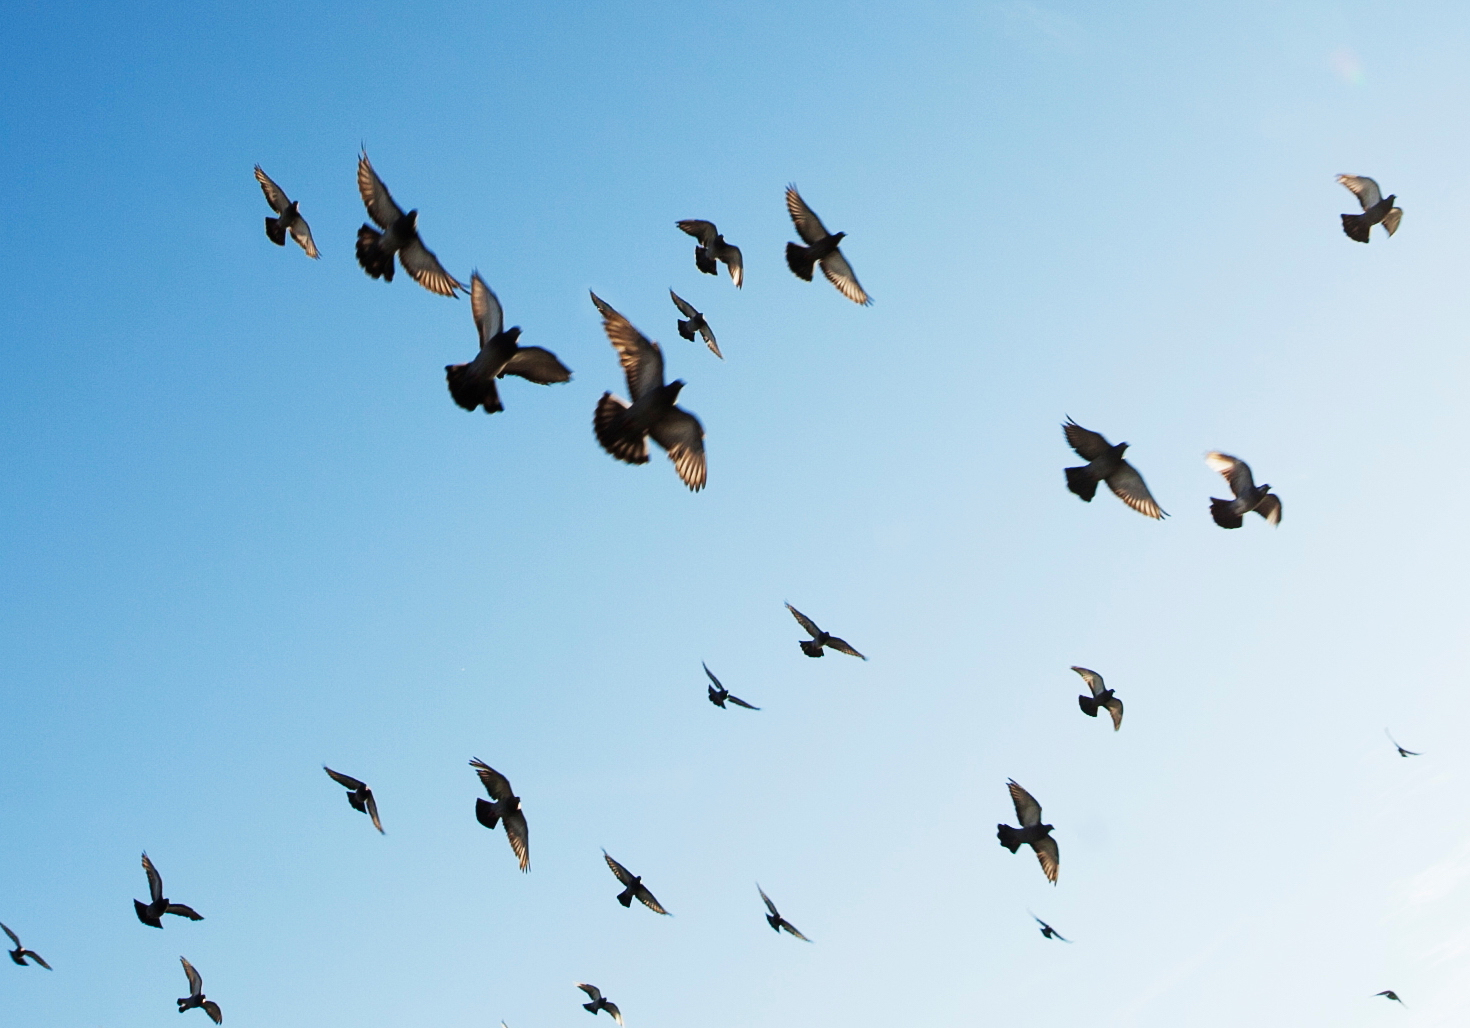
\includegraphics[width=1\linewidth]{figures/pyramids/birds_multiscale.jpg}
%}
%\caption{Scale invariance is a fundamental property of images. Objects in images appear at arbitrary locations (translation invariance) and with arbitrary image sizes (scale invariance). Scale changes are a consequence of perspective projection.}
%\label{fig:birds_multiscale}
%\end{figure}
%

%In the previous chapters we have seen the power of simple linear filters to extract useful image properties. Things get a lot more interesting when many filters are used in order to represent images. In this chapter we will study some important filter ensembles. 

%We will focus on the following properties:
%\begin{itemize}
%\item Multiscale image analysis
%\item Reconstruction property
%\item Non-aliased representations
%\end{itemize}
%

% Basic references:
% http://users.utcluj.ro/~tmarita/HCI/C7-8-extra/Pyramids/RCA84.pdf

%Which properties should a filter set have?

In chapter XX we motivated translation invariant linear filters as a way of accounting for the fact that objects in images might appear at any location. Therefore, a reasonable way of processing an image is by manipulating pixel neighborhoods  in the same way independently on the image location. In addition to translation invariance, scale invariance is another fundamental property of images. Due to perspective projection, objects at different distances will appear with different sizes as shown in figure~\ref{fig:birds_multiscale_processing}. Therefore, if we want to locate all the bird instances in this image, we will have to apply an operator that is invariant in translation and in scale. Image pyramids provide an efficient representation for space-scale invariant processing.

\section{Image Pyramids and multi-scale image analysis}

\begin{figure}
\centerline{
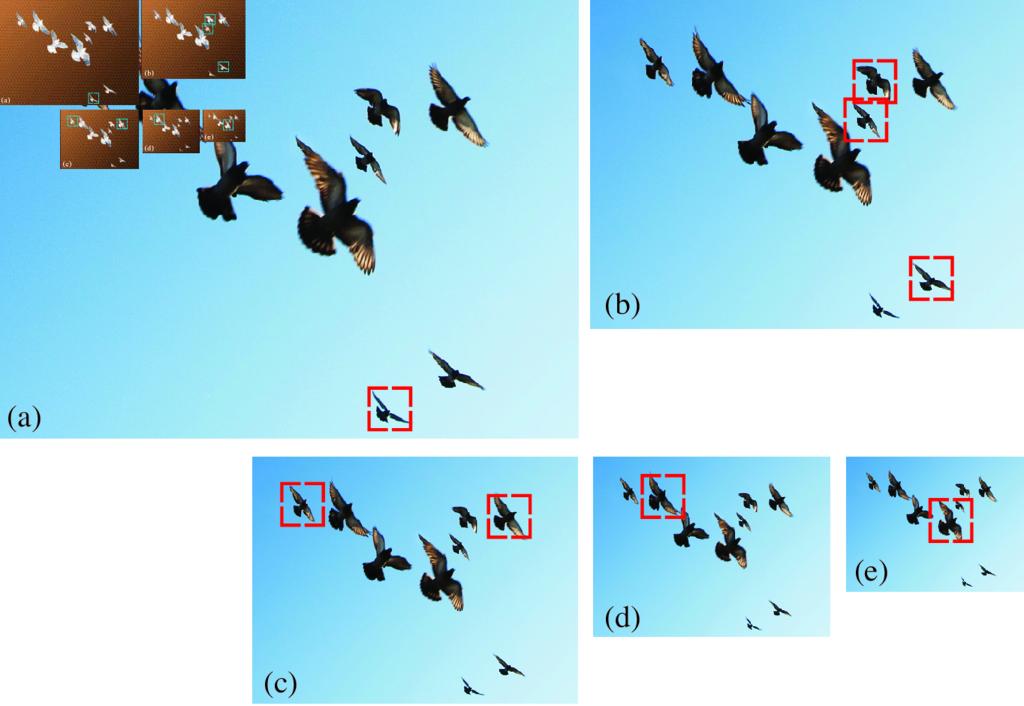
\includegraphics[width=.8\linewidth]{figures/pyramids/multiscale_birds_boxes.eps}
}
\caption{Multiscale image pyramid. Each image is 25$\%$ smaller than the previous one. The red box indicates the size of a template used for detecting flying birds. As the size of the template is fixed, it will only be able to detect the birds that tightly fit inside the box. Birds that are smaller or larger will not be detected within a single scale. By running the same template across many levels in this pyramid, different birds instances are detected at different scales.}
\label{fig:birds_multiscale_processing}
\end{figure}


Image information occurs over many different spatial scales.
Image pyramids--multi-resolution representations for images--are a
useful data structure for analyzing and manipulating images over a
range of spatial scales.  Here we'll discuss three different ones, in a
progression of complexity. The first is a Gaussian pyramid, which creates versions of the input
image at multiple resolutions.  This is useful for analysis across
different spatial scales, but doesn't separate the image into
different frequency bands.  The Laplacian pyramid provides that extra
level of analysis, breaking the image into different isotropic spatial
frequency bands.  
%The Wavelet or QMF (quadrature mirror filter)
%pyramid provides some splitting of the spatial frequency bands
%according to orientation (although in a somewhat limited way).  
The
Steerable pyramid provides a clean separation of the image into
different scales and orientations.  There are various other
differences between these pyramids, which we'll describe below.


As a motivating example, lets assume we want to detect the birds from figure~\ref{fig:birds_multiscale} using the normalized correlation approach described in section XX. If we have a template of a bird, the normalized correlation will be able to detect only the birds that have a similar image size than the template. To introduce scale invariance, one possible solution is to change the size of the template to cover a wide range of possible sizes and apply them to the image. Then, the ensemble of templates will be able to detect birds of different sizes. The disadvantage of this approach is that it will be computationally expensive as detecting large birds will require computing convolutions with big kernels which is very slow. Another alternative is to change the image size as shown in figure~\ref{fig:birds_multiscale_processing} resulting in a {\em multiscale image pyramid}. In this example, the original image has a resolution of 848$\times$643 pixels. Each image in the pyramid is obtained by scaling down the image from the previous level by reducing the number of pixels by factor of $25\%$. This operation is called downsampling and we will study it in detail in this chapter. Now we can use the pyramid to detect birds at different sizes using a single template. The red box in the figure denotes the size of the template used. The figure shows how birds of different sizes become detectable at, at least, one of the levels of the pyramid. This method will be more efficient as the template can be kept small and the convolutions will remain computationally efficient. 

Mutiscale image processing and image pyramids have many applications beyond scale invariant object detection. In this chapter we will describe some important image pyramids and their applications. 


\section{Linear image transforms}

Let's first look at some general properties of linear image transforms.  For an input image $x$ of $N$ pixels, a linear transform is:
\begin{equation}
r = P^T x 
\end{equation}
where $r$ is a vector of dimensionality $M$, and $P$ is  a matrix of size $N \times M$. The columns of $P = \left[P_0,  P_1, ...,P_{M-1}\right]$ are the projection vectors. The vector $r$ contains the transform coefficients: $r_i = P_i^T x$.  The vector $r$ corresponds to a different representation of the image $x$ than the original pixel space. 

The transform $P$ is said to be critically sampled when $M=N$.  The transform is over-sampled when $M > N$, and under-sampled when $M < N$. We are interested in transforms that are invertible, so that we can recover the input $x$ from the projection coefficients $r$:
\begin{equation}
x = B r = \sum_{i=0}^{M-1} r_i B_i 
\end{equation}
The columns of $B= \left[B_0,  B_1, ...,B_{M-1}\right]$ are the basis vectors. The input signal $x$ can be reconstructed as a linear combination of the basis vectors $B_i$ weighted by the representation coefficients $r_i$.  

The transform $P$ is complete, encoding all image structure, if it is invertible. If critically sampled (i.e., $M=N$) and the transform is complete, then $B = (P^T)^{-1}$.  If it is over-complete (over-sampled and complete), then the inverse can be obtained using the pseudo inverse $B=(P P^T)^{-1}P$.

An important special case is when the transform is self-inverting, then $P P^{T} = I$. The values of $P$ can be real  or complex (like in the Fourier transform). For complex transforms, we should replace the $P^T$ by $P^{*T}$ (complex conjugate transpose).




\section{Gaussian pyramid}


%
%
%
%\begin{figure}
%\centerline{
%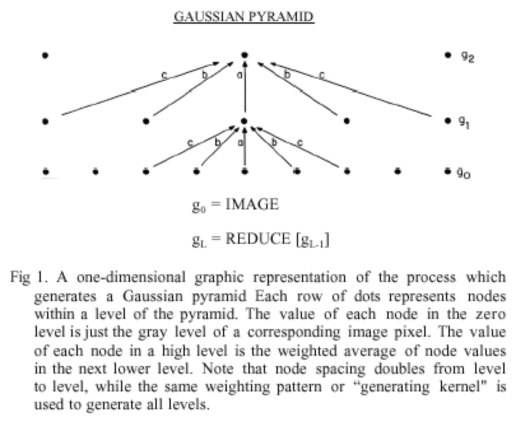
\includegraphics[width=0.7\linewidth]{figures/pyramids/gausspyr.jpg}
%}
%\caption{Computation for the Gaussian pyramid.}
%\label{fig:gausspyr}
%\end{figure}
%
%
%\begin{figure}
%\centerline{
%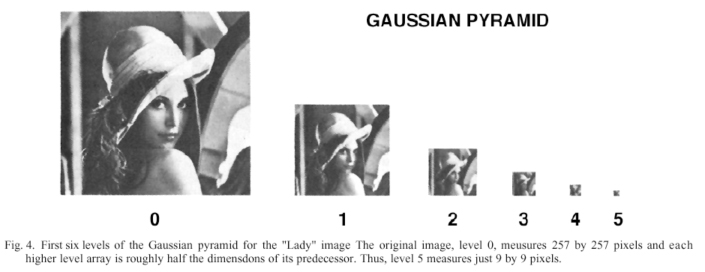
\includegraphics[width=0.8\linewidth]{figures/pyramids/gpyr.jpg}
%}
%\caption{Gaussian pyramid example}
%\label{fig:gpyr}
%\end{figure}
%
%
%\begin{figure}
%\centerline{
%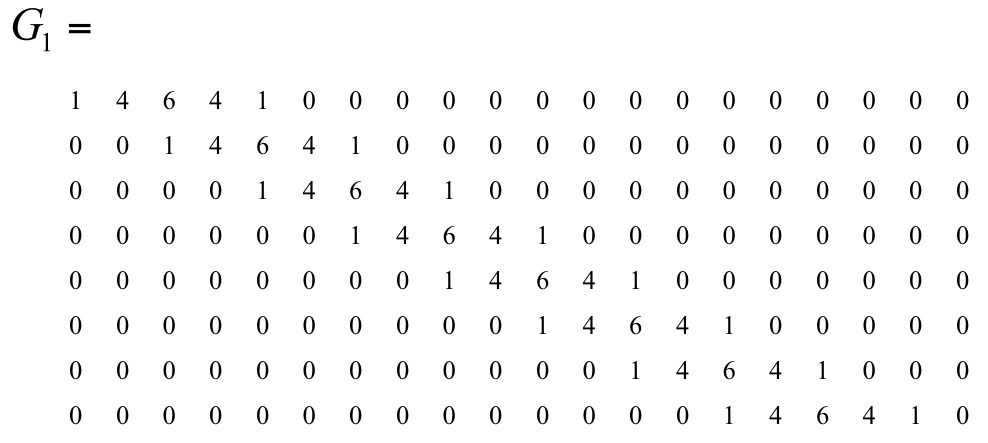
\includegraphics[width=0.8\linewidth]{figures/pyramids/gpnums1.jpg}
%}
%\centerline{
%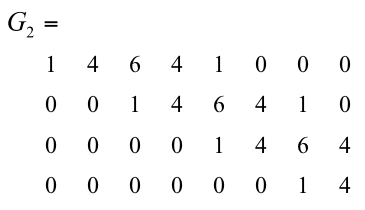
\includegraphics[width=0.4\linewidth]{figures/pyramids/gpnums2.jpg}
%}
%\centerline{
%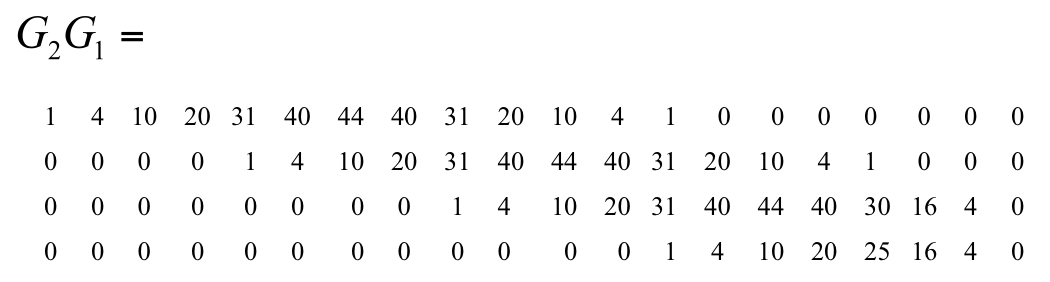
\includegraphics[width=0.8\linewidth]{figures/pyramids/gpnums3.jpg}
%}
%\caption{Gaussian pyramid matrix numbers}
%\label{fig:gpnums}
%\end{figure}


We'd like to make a recursive algorithm for creating a multi-resolution version of an image.  A gaussian filter is a natural
one to use to blur out an image, since multiple applications of a gaussian filter is equivalent to application of a single, wider
gaussian filter.

Here's an elegant, efficient algorithm for making a resolution reduced version of an input image.  It involves two steps:  convolving the
image with a low-pass filter (for example, using the 4-th binomial filter $b_4 = [1, 4, 6, 4, 1]$ / 16, normalized to sum to 1, separably in each dimension), and then subsampling by a factor of 2 the result. Each level is obtained by filtering the previous level with the 4-th binomial filter with a stride of 2 (on each dimension). Applied recursively, this algorithm generates a sequence of images,  subsequent ones being smaller, lower resolution versions of the earlier ones in the processing.
% Drawing the blocks of first level:
\marginnote{One {\bf block} of the Gaussian pyramid computation.
\\~\\
\tikzset{
  block/.style    = {draw, thin, rectangle, minimum height = 1.5em,  minimum width = 1.5em},
  sum/.style      = {draw, circle, minimum size=.4cm}, % Adder
  input/.style    = {coordinate}, % Input
  output/.style   = {coordinate}, % Output
  x/.style   = {coordinate} % Output
}
\begin{tikzpicture}[auto, thin, node distance=1.2cm, >=triangle 45]
\draw
	node [input] (x0) {}
	node [right of=x0, node distance=0cm] (x0p) {$g_k$}
	%node [input] (x0p) {$x_0$}
	node [block, right of=x0p] (g0) {$G_k$}
	node [right of=g0] (x1) {$g_{k+1}$};
       % Joining blocks. 
	%\draw[-](x0) -- node {} (x0p);
	\draw[->](x0p) -- node {} (g0);
	\draw[->](g0) -- node {} (x1);
	%\draw [->] (a3) -| node[pos=0.99, right] {{\tiny $-$}} (sum);
\end{tikzpicture}
}

To make the filters more intuitive, it is useful to write the two steps in matrix form. The following matrix shows the recursive construction of  level $k+1$ of the Gaussian pyramid for a 1D image:
\begin{equation}
g_{k+1} = D_k B_k g_k = G_k g_k
\end{equation}
where $D_k$ is the downsampling operator, $B_k$ is the convolution with the 4-th binomial filter, and $G_k = D_kB_k$ is the blur-and-downsample operator for level $k$. We call the  sequence of images  $g_0,  g_1, . . ., g_N$  as the Gaussian pyramid.  The first level of the Gaussian pyramid is the input image: $g_0=x$.


It is useful to check a concrete example. If $x$ is a 1D signal of length 8, and if we assume zero boundary conditions, the matrices for computing $g_1$ are:
\begin{equation}
G_0 = D_0 B_0 =
\begin{bmatrix}
  1 ~& 0 ~& 0 ~& 0 ~& 0 ~& 0 ~& 0 ~& 0 \\
  0 ~& 0 ~& 1 ~& 0 ~& 0 ~& 0 ~& 0 ~& 0 \\
  0 ~& 0 ~& 0 ~& 0 ~& 1 ~& 0 ~& 0 ~& 0 \\
  0 ~& 0 ~& 0 ~& 0 ~& 0 ~& 0 ~& 1 ~& 0
 \end{bmatrix}
 \frac{1}{16}
 \begin{bmatrix}
  6 ~& 4 ~& 1 ~& 0 ~& 0 ~& 0 ~& 0 ~& 0 \\
  4 ~& 6 ~& 4 ~& 1 ~& 0 ~& 0 ~& 0 ~& 0 \\
  1 ~& 4 ~& 6 ~& 4 ~& 1 ~& 0 ~& 0 ~& 0 \\
  0 ~& 1 ~& 4 ~& 6 ~& 4 ~& 1 ~& 0 ~& 0 \\
  0 ~& 0 ~& 1 ~& 4 ~& 6 ~& 4 ~& 1 ~& 0 \\
  0 ~& 0 ~& 0 ~& 1 ~& 4 ~& 6 ~& 4 ~& 1 \\
  0 ~& 0 ~& 0 ~& 0 ~& 1 ~& 4 ~& 6 ~& 4 \\
  0 ~& 0 ~& 0 ~& 0 ~& 0 ~& 1 ~& 4 ~& 6 
\end{bmatrix}
\end{equation}
Multiplying the two matrices:
\begin{equation}
g_{1} = G_0 x = 
 \frac{1}{16}
 \begin{bmatrix}
  6 ~& 4 ~& 1 ~& 0 ~& 0 ~& 0 ~& 0 ~& 0 \\
  1 ~& 4 ~& 6 ~& 4 ~& 1 ~& 0 ~& 0 ~& 0 \\
  0 ~& 0 ~& 1 ~& 4 ~& 6 ~& 4 ~& 1 ~& 0 \\
  0 ~& 0 ~& 0 ~& 0 ~& 1 ~& 4 ~& 6 ~& 4 
 \end{bmatrix}
 x
 \end{equation}
the first level of the gaussian pyramid is a signal $g_1$ with length 4. Applying the recursion we can write the output of each level as a function of the input $x$:  $g_{2} = G_1 G_0 x$, $g_{3} = G_2 G_1 G_0 x$, and so on. 
 
For 2D images the operations are analogous. Figure~\ref{fig:gausspyr} shows the Gaussian pyramid of an image. 


\begin{figure}[h!]
\centerline{
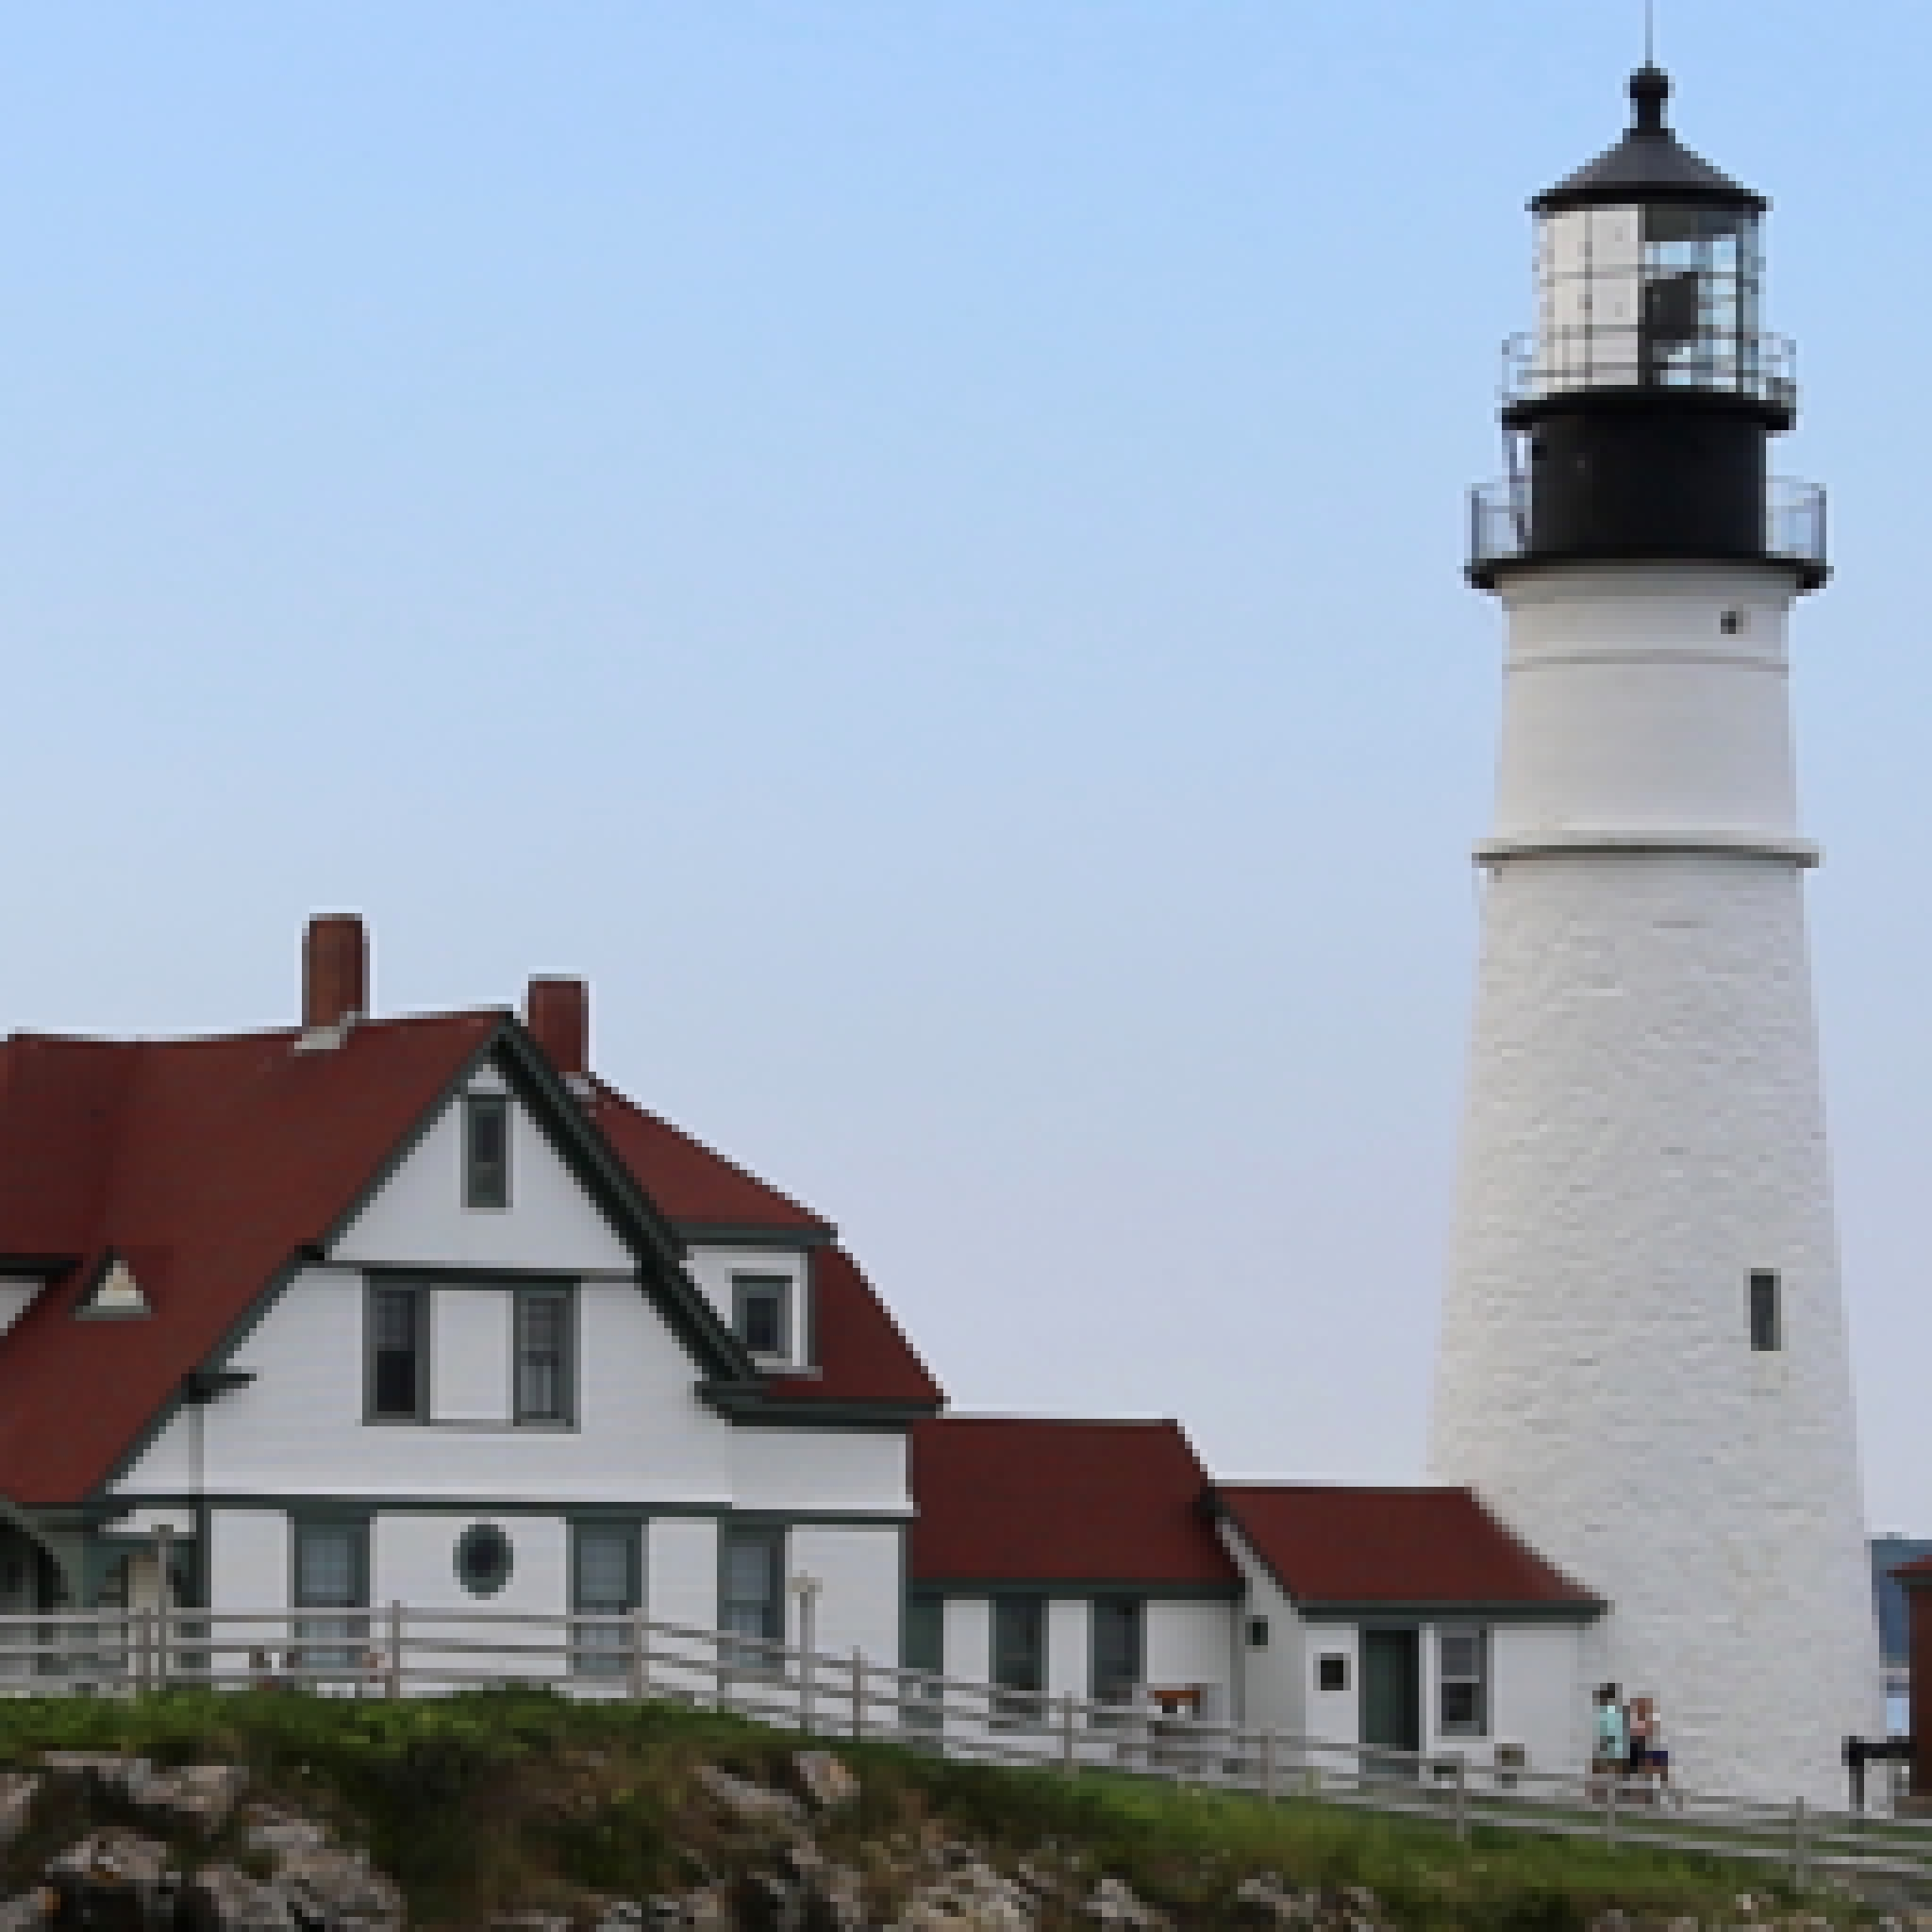
\includegraphics[width=0.5\linewidth]{figures/pyramids/gaussianPyr_1.jpg}
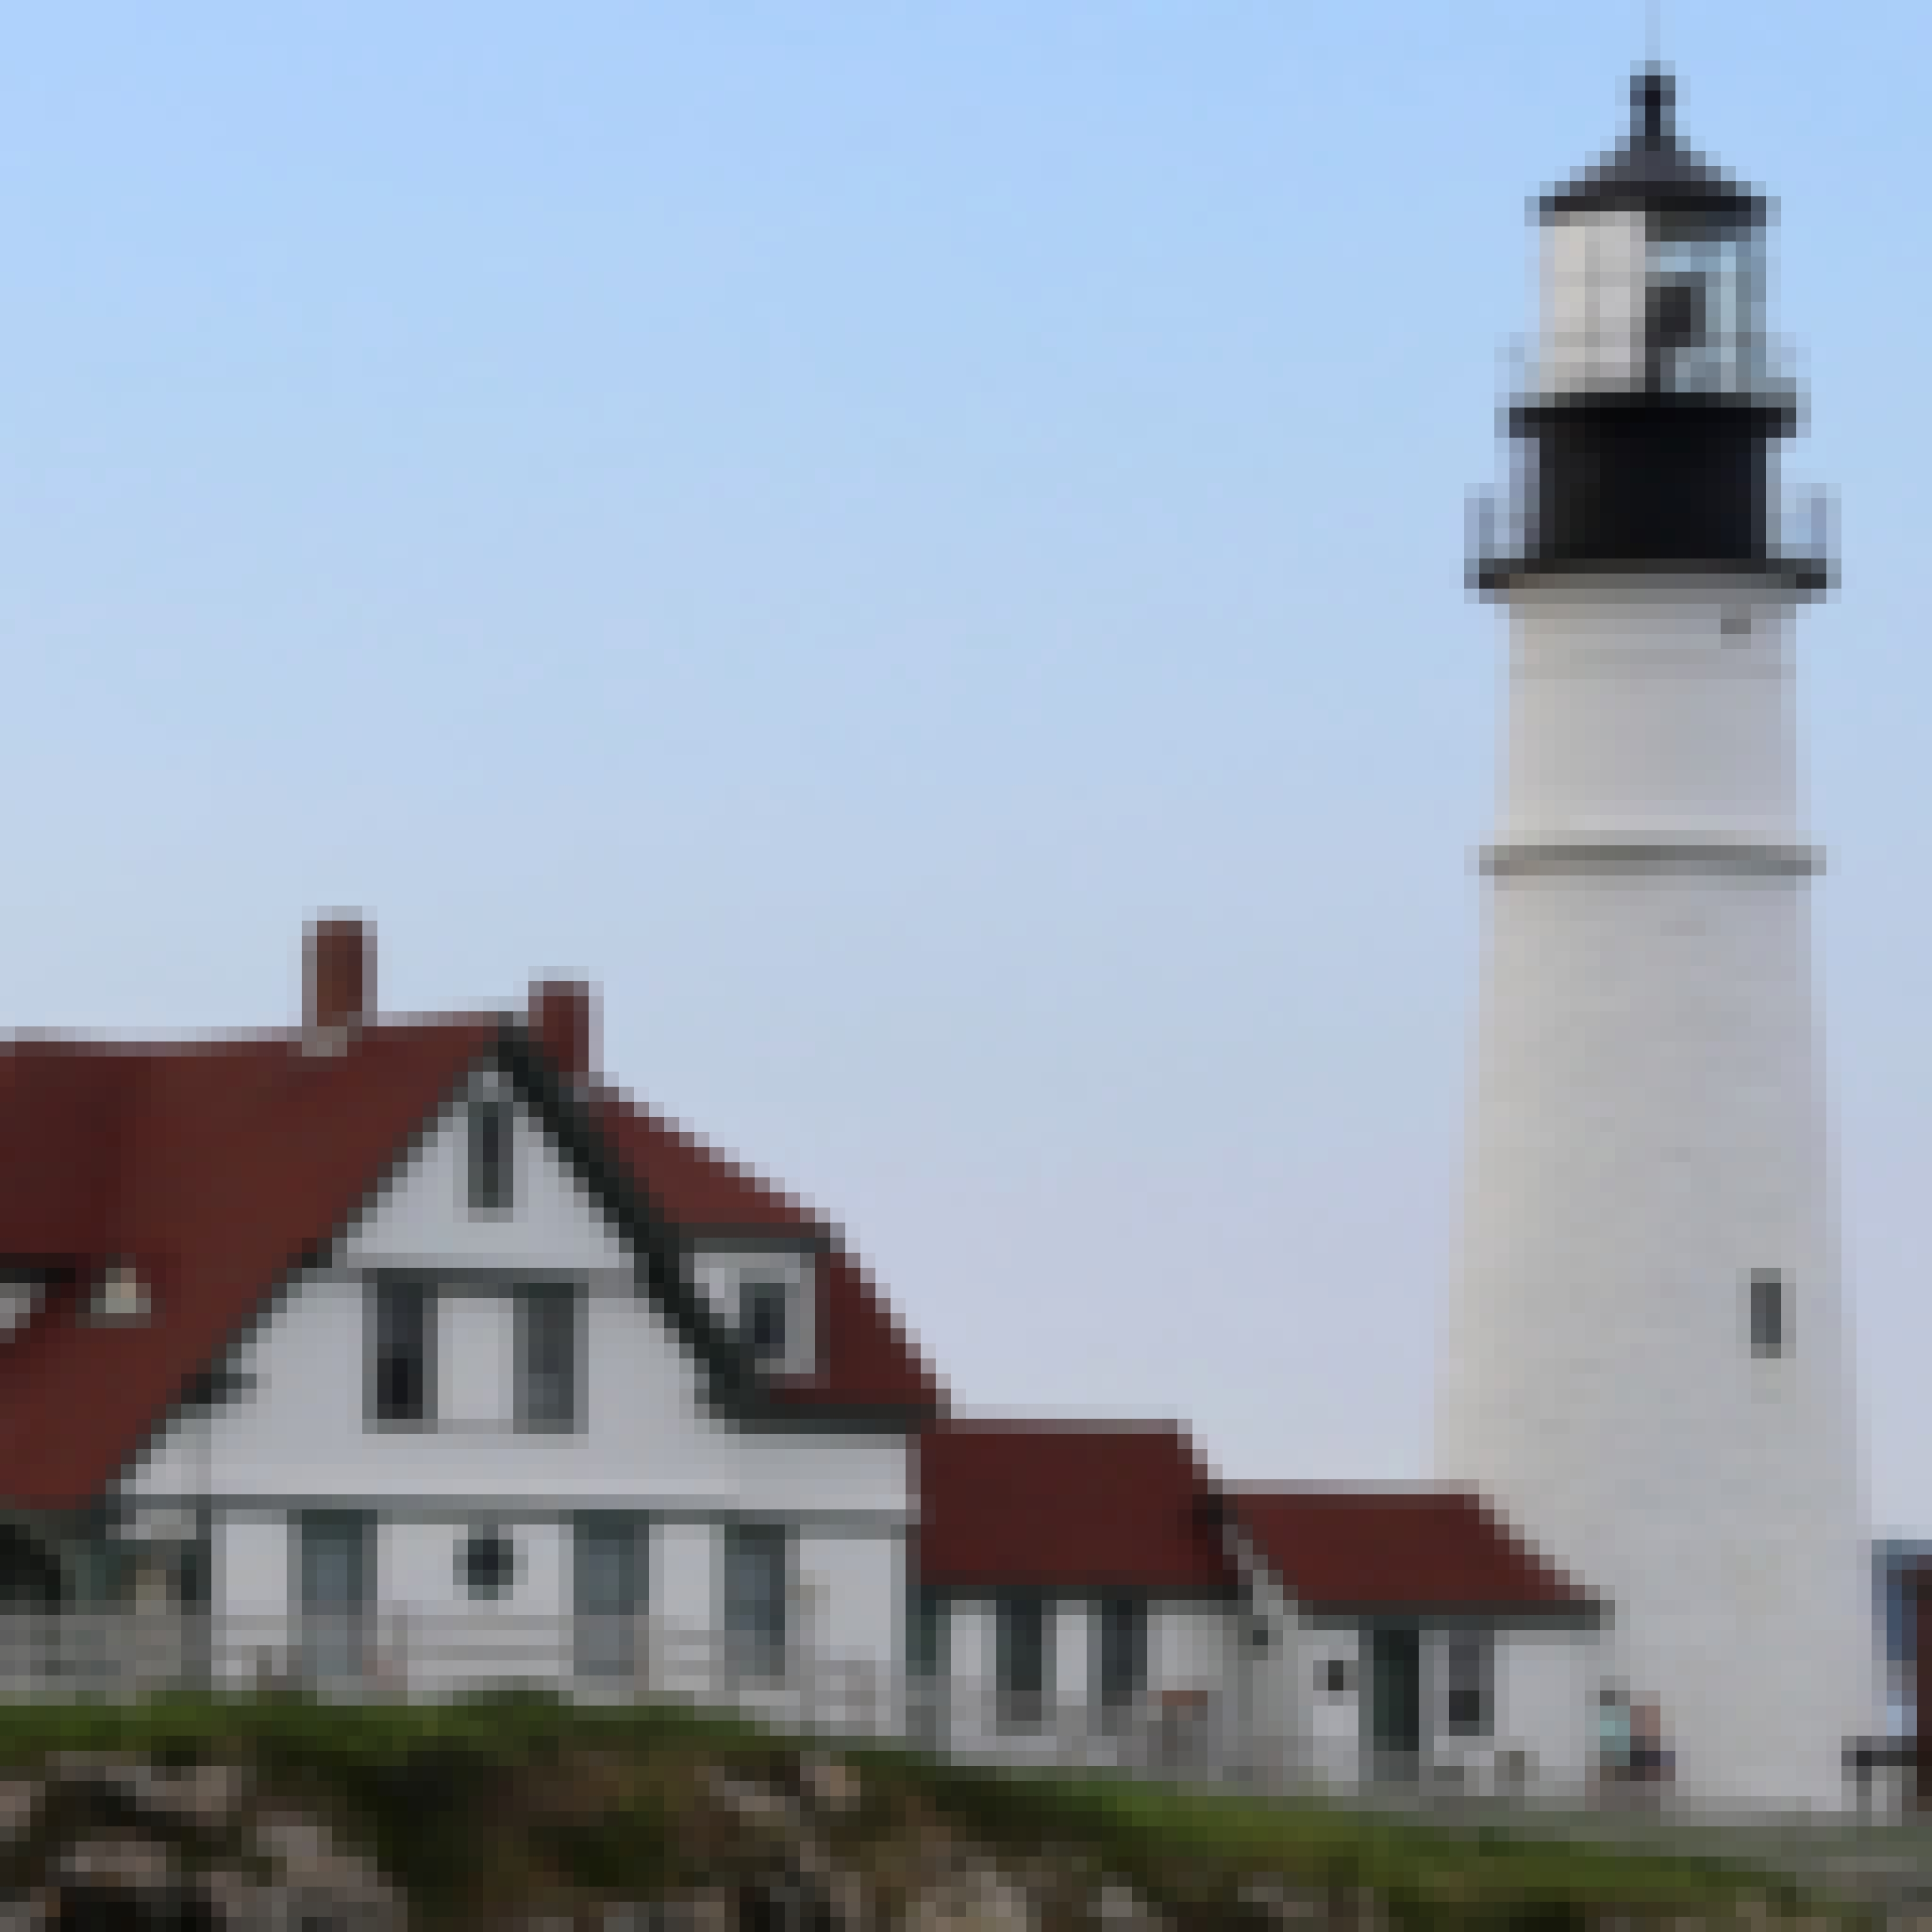
\includegraphics[width=0.25\linewidth]{figures/pyramids/gaussianPyr_2.jpg}

\includegraphics[width=0.125\linewidth]{figures/pyramids/gaussianPyr_3.jpg}
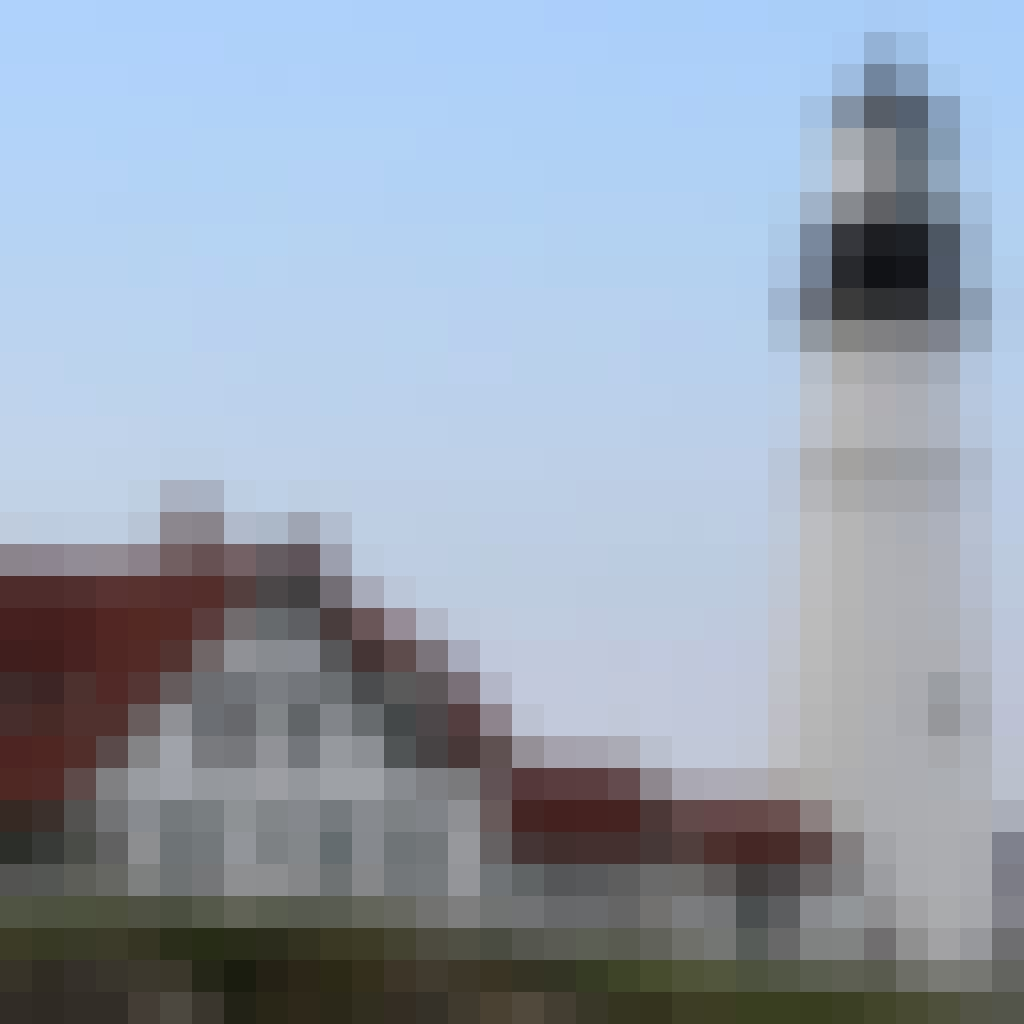
\includegraphics[width=0.0625\linewidth]{figures/pyramids/gaussianPyr_4.jpg}

\includegraphics[width=0.03125\linewidth]{figures/pyramids/gaussianPyr_5.jpg}

\includegraphics[width=0.015625\linewidth]{figures/pyramids/gaussianPyr_6.jpg}
}
\caption{Gaussian pyramid. The Gaussian pyramid is built for each color channel independently.}
\label{fig:gausspyr}
\end{figure}


%
%
%Fig.~\ref{fig:gpnums} shows a matrix which shows the contributions of each
%pixel of a (1-d) image in the Gaussian pyramid image two levels above
%it in the pyramid.  Note the large spatial extent of the low-pass
%filtering, but accomplished much more efficiently than a naive
%filtering with the equivalent low-pass filter all in one step.
%
%The Gaussian pyramid is useful for coarse-to-fine processing of
%images--using analysis at a coarse resolution to initialize processing
%at a finer level of detail.  This is shown in Fig.~\ref{fig:gpyr}.

%
%\begin{figure}
%\centerline{
%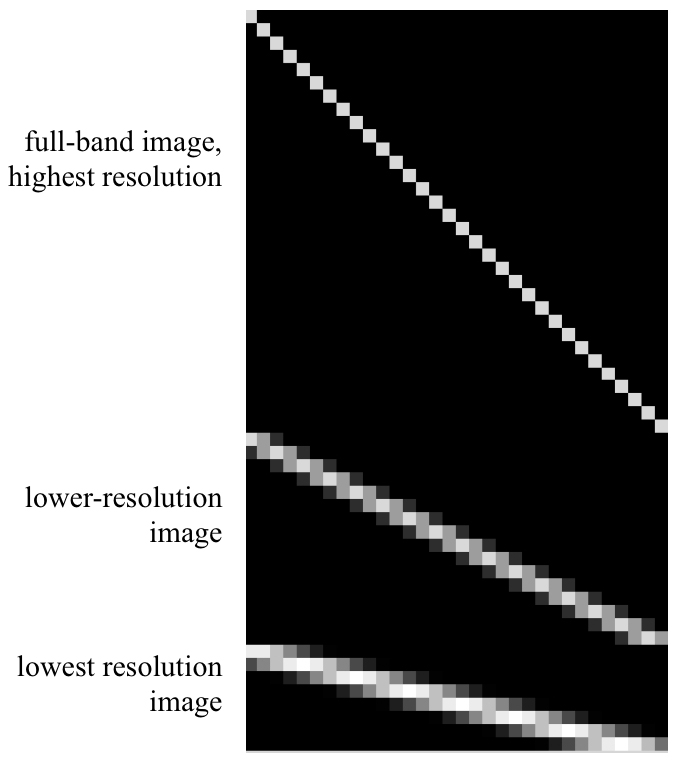
\includegraphics[width=0.5\linewidth]{figures/pyramids/gpyrmat.jpg}
%}
%\caption{Gaussian pyramid matrix image}
%\label{fig:gpyrmat}
%\end{figure}
%
%

%Fig.~\ref{fig:gpyrmat}
%shows the equivalent matrix for a simple, 3-level Gaussian pyramid
%(the pyramid is actually constructed more efficiently than by performing
%this matrix multiplication).    This matrix generates 3 versions of
%the image:  one a full resolution, a second at half the (linear) resolution,
%and a 3rd at 1/4 the resolution of the original.

\section{Laplacian pyramid}

In the gaussian pyramid, each level losses some of the fine image details available in the previous level. %The goal of the Laplacian pyramid is to represent, at each level, what is present in a Gaussian pyramid image of one level, but not present at the level below it. 
The Laplacian pyramid is simple:  it represents, at each level, what
is present in a Gaussian pyramid image of one level, but not present
at the level below it.  We calculate that by expanding the
lower-resolution Gaussian pyramid image to the same pixel resolution
as the neighboring higher-resolution Gaussian pyramid image, then
subtracting the two.  This calculation is made in a recursive,
telescoping fashion. 




% Drawing the blocks of first level:
\marginnote{One {\bf block} of the Laplacian pyramid computation.
\\~\\
\tikzset{
  block/.style    = {draw, thin, rectangle, minimum height = 1.5em,  minimum width = 1.5em},
  sum/.style      = {draw, circle, minimum size=.4cm}, % Adder
  input/.style    = {coordinate}, % Input
  output/.style   = {coordinate}, % Output
  x/.style   = {coordinate} % Output
}
\begin{tikzpicture}[auto, thin, node distance=1.2cm, >=triangle 45]
\draw
	node [input] (x0) {}
	node [right of=x0, node distance=0cm] (x0p) {$g_k$}
	%node [input] (x0p) {$x_0$}
	node [block, right of=x0p] (g0) {$G_k$}
        node [block, below of=g0] (f0) {$F_k$}
	node [sum, left of=f0] (suma0) {}
	node [right of=g0] (x1) {$g_{k+1}$}
	node [below of=suma0] (l0) {$l_k$};
       % Joining blocks. 
	%\draw[-](x0) -- node {} (x0p);
	\draw[->](x0p) -- node {} (g0);
	\draw[->](x0p) -- node[pos=0.99, left] {{\tiny $+$}} (suma0);
	\draw[->](f0) -- node[pos=0.99, below] {{\tiny $-$}} (suma0);
	\draw[->](x1) |- node {} (f0);
	\draw[->](g0) |- node {} (x1);
	\draw[->](suma0) -- node {} (l0);
	%\draw [->] (a3) -| node[pos=0.99, right] {{\tiny $-$}} (sum);
\end{tikzpicture}
}

Let's look at the steps for calculating a Laplacian pyramid.
What we want is to compute the difference between $g_k$ and  $g_{k+1}$. To do this first we need to upsample the image $g_{k+1}$ so that it has the same size as $g_k$. Let $F_k = B_k U_k$ be the upsample-and-blur operator for pyramid level $k$.  The operator $F_k$ applies first the upsampling operator $U_k$, that inserts zeros between samples, followed by blurring by the same filter $B_k$ than the one we used for the Gaussian pyramid. The Laplacian pyramid coefficients, $l_k$, at pyramid level $k$, are:  
%% we must interpolate the image
%% back up to full size before subtracting it from the original.  The
%% upConv function does upsampling (padding with zeros between
%% samples) followed by convolution.  This can be done using the
%% lowpass filter that was applied before subsampling or it can be
%% done with a different filter.
%\begin{equation}
%L_n = (I_n - F_n G_n) x_n,
%\end{equation}
\begin{equation}
l_{k} =  g_k - F_k g_{k+1} =  (I_k - F_k G_k) g_{k} 
\end{equation}

For instance, for a 1D input $x$ of length 8, and assuming zero boundary conditions, the operators to compute the first level of the Laplacian pyramid are:
\begin{equation}
F_0 =  2 B_0 U_0 =
 \frac{1}{8}
 \begin{bmatrix}
  6 ~& 4 ~& 1 ~& 0 ~& 0 ~& 0 ~& 0 ~& 0 \\
  4 ~& 6 ~& 4 ~& 1 ~& 0 ~& 0 ~& 0 ~& 0 \\
  1 ~& 4 ~& 6 ~& 4 ~& 1 ~& 0 ~& 0 ~& 0 \\
  0 ~& 1 ~& 4 ~& 6 ~& 4 ~& 1 ~& 0 ~& 0 \\
  0 ~& 0 ~& 1 ~& 4 ~& 6 ~& 4 ~& 1 ~& 0 \\
  0 ~& 0 ~& 0 ~& 1 ~& 4 ~& 6 ~& 4 ~& 1 \\
  0 ~& 0 ~& 0 ~& 0 ~& 1 ~& 4 ~& 6 ~& 4 \\
  0 ~& 0 ~& 0 ~& 0 ~& 0 ~& 1 ~& 4 ~& 6 
\end{bmatrix}
 \begin{bmatrix}
  1 ~& 0 ~& 0  ~& 0\\
  0 ~& 0 ~& 0  ~& 0\\
  0 ~& 1 ~& 0  ~& 0\\
  0 ~& 0 ~& 0  ~& 0\\
  0 ~& 0 ~& 1  ~& 0\\
  0 ~& 0 ~& 0  ~& 0\\
  0 ~& 0 ~& 0  ~& 1\\
  0 ~& 0 ~& 0  ~& 0
\end{bmatrix}
 \end{equation}
The factor 2 is necessary because inserting zeros decreases the average value of the signal $g_{k+1}$ by a factor of 2. Multiplying the two matrices:
\begin{equation}
l_{0} = g_0 - F_0 g_{1} = 
 g_0 - \frac{1}{8}
 \begin{bmatrix}
  6 ~& 1 ~& 0  ~& 0\\
  4 ~& 4 ~& 0  ~& 0\\
  1 ~& 6 ~& 1  ~& 0\\
  0 ~& 4 ~& 4  ~& 0\\
  0 ~& 1 ~& 6  ~& 1\\
  0 ~& 0 ~& 4  ~& 4\\
  0 ~& 0 ~& 1  ~& 6\\
  0 ~& 0 ~& 0  ~& 4
\end{bmatrix}
 g_{1}
 \end{equation}
We can also calculate the matrix that should be applied to the input$x=g_0$.
\begin{equation}
l_{0} =  (I - F_0 G_0) g_0= 
\frac{1}{256}
 \begin{bmatrix}
   182 ~& -56  ~& -24 ~&   -8   ~& -2  ~&   0  ~&   0  ~&   0\\
   -56  ~& 192  ~& -56 ~&  -32   ~& -8   ~&  0  ~&   0   ~&  0\\
   -24  ~& -56  ~& 180  ~& -56 ~&  -24  ~&  -8  ~&  -2   ~&  0\\
    -8   ~&-32  ~& -56  ~& 192  ~& -56  ~& -32  ~&  -8   ~&  0\\
    -2   ~& -8 ~&  -24  ~& -56 ~&  180 ~&  -56  ~& -24 ~&   -8\\
     0   ~&  0  ~&  -8  ~& -32 ~&  -56  ~& 192  ~& -56  ~& -32\\
     0   ~&   0  ~&  -2  ~&  -8  ~& -24  ~& -56 ~&  182  ~& -48\\
     0   ~&   0   ~&  0  ~&   0   ~& -8  ~& -32 ~&  -48 ~&  224
\end{bmatrix}
x
\end{equation}



\begin{figure}
\centerline{
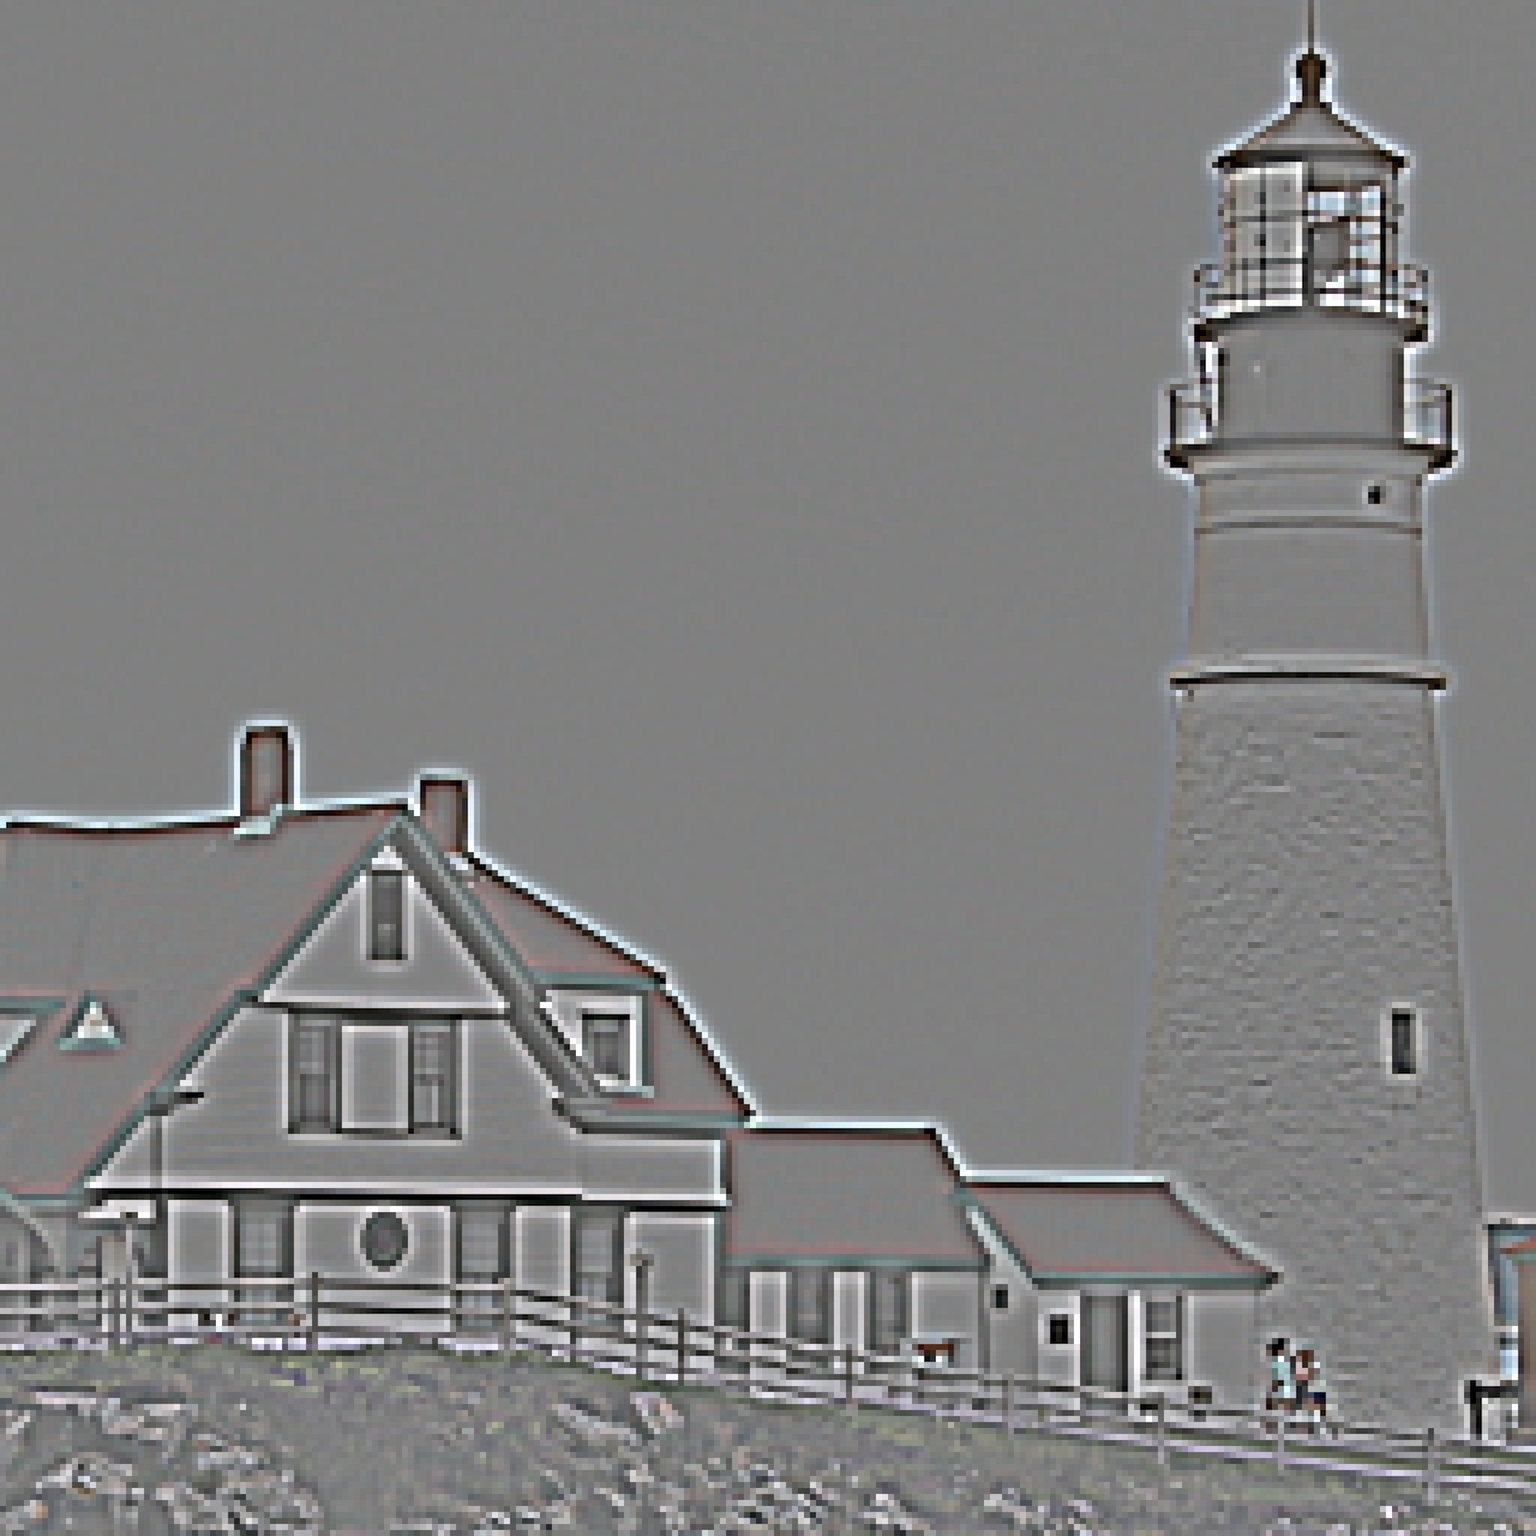
\includegraphics[width=0.5\linewidth]{figures/pyramids/laplacianPyr_1.jpg}
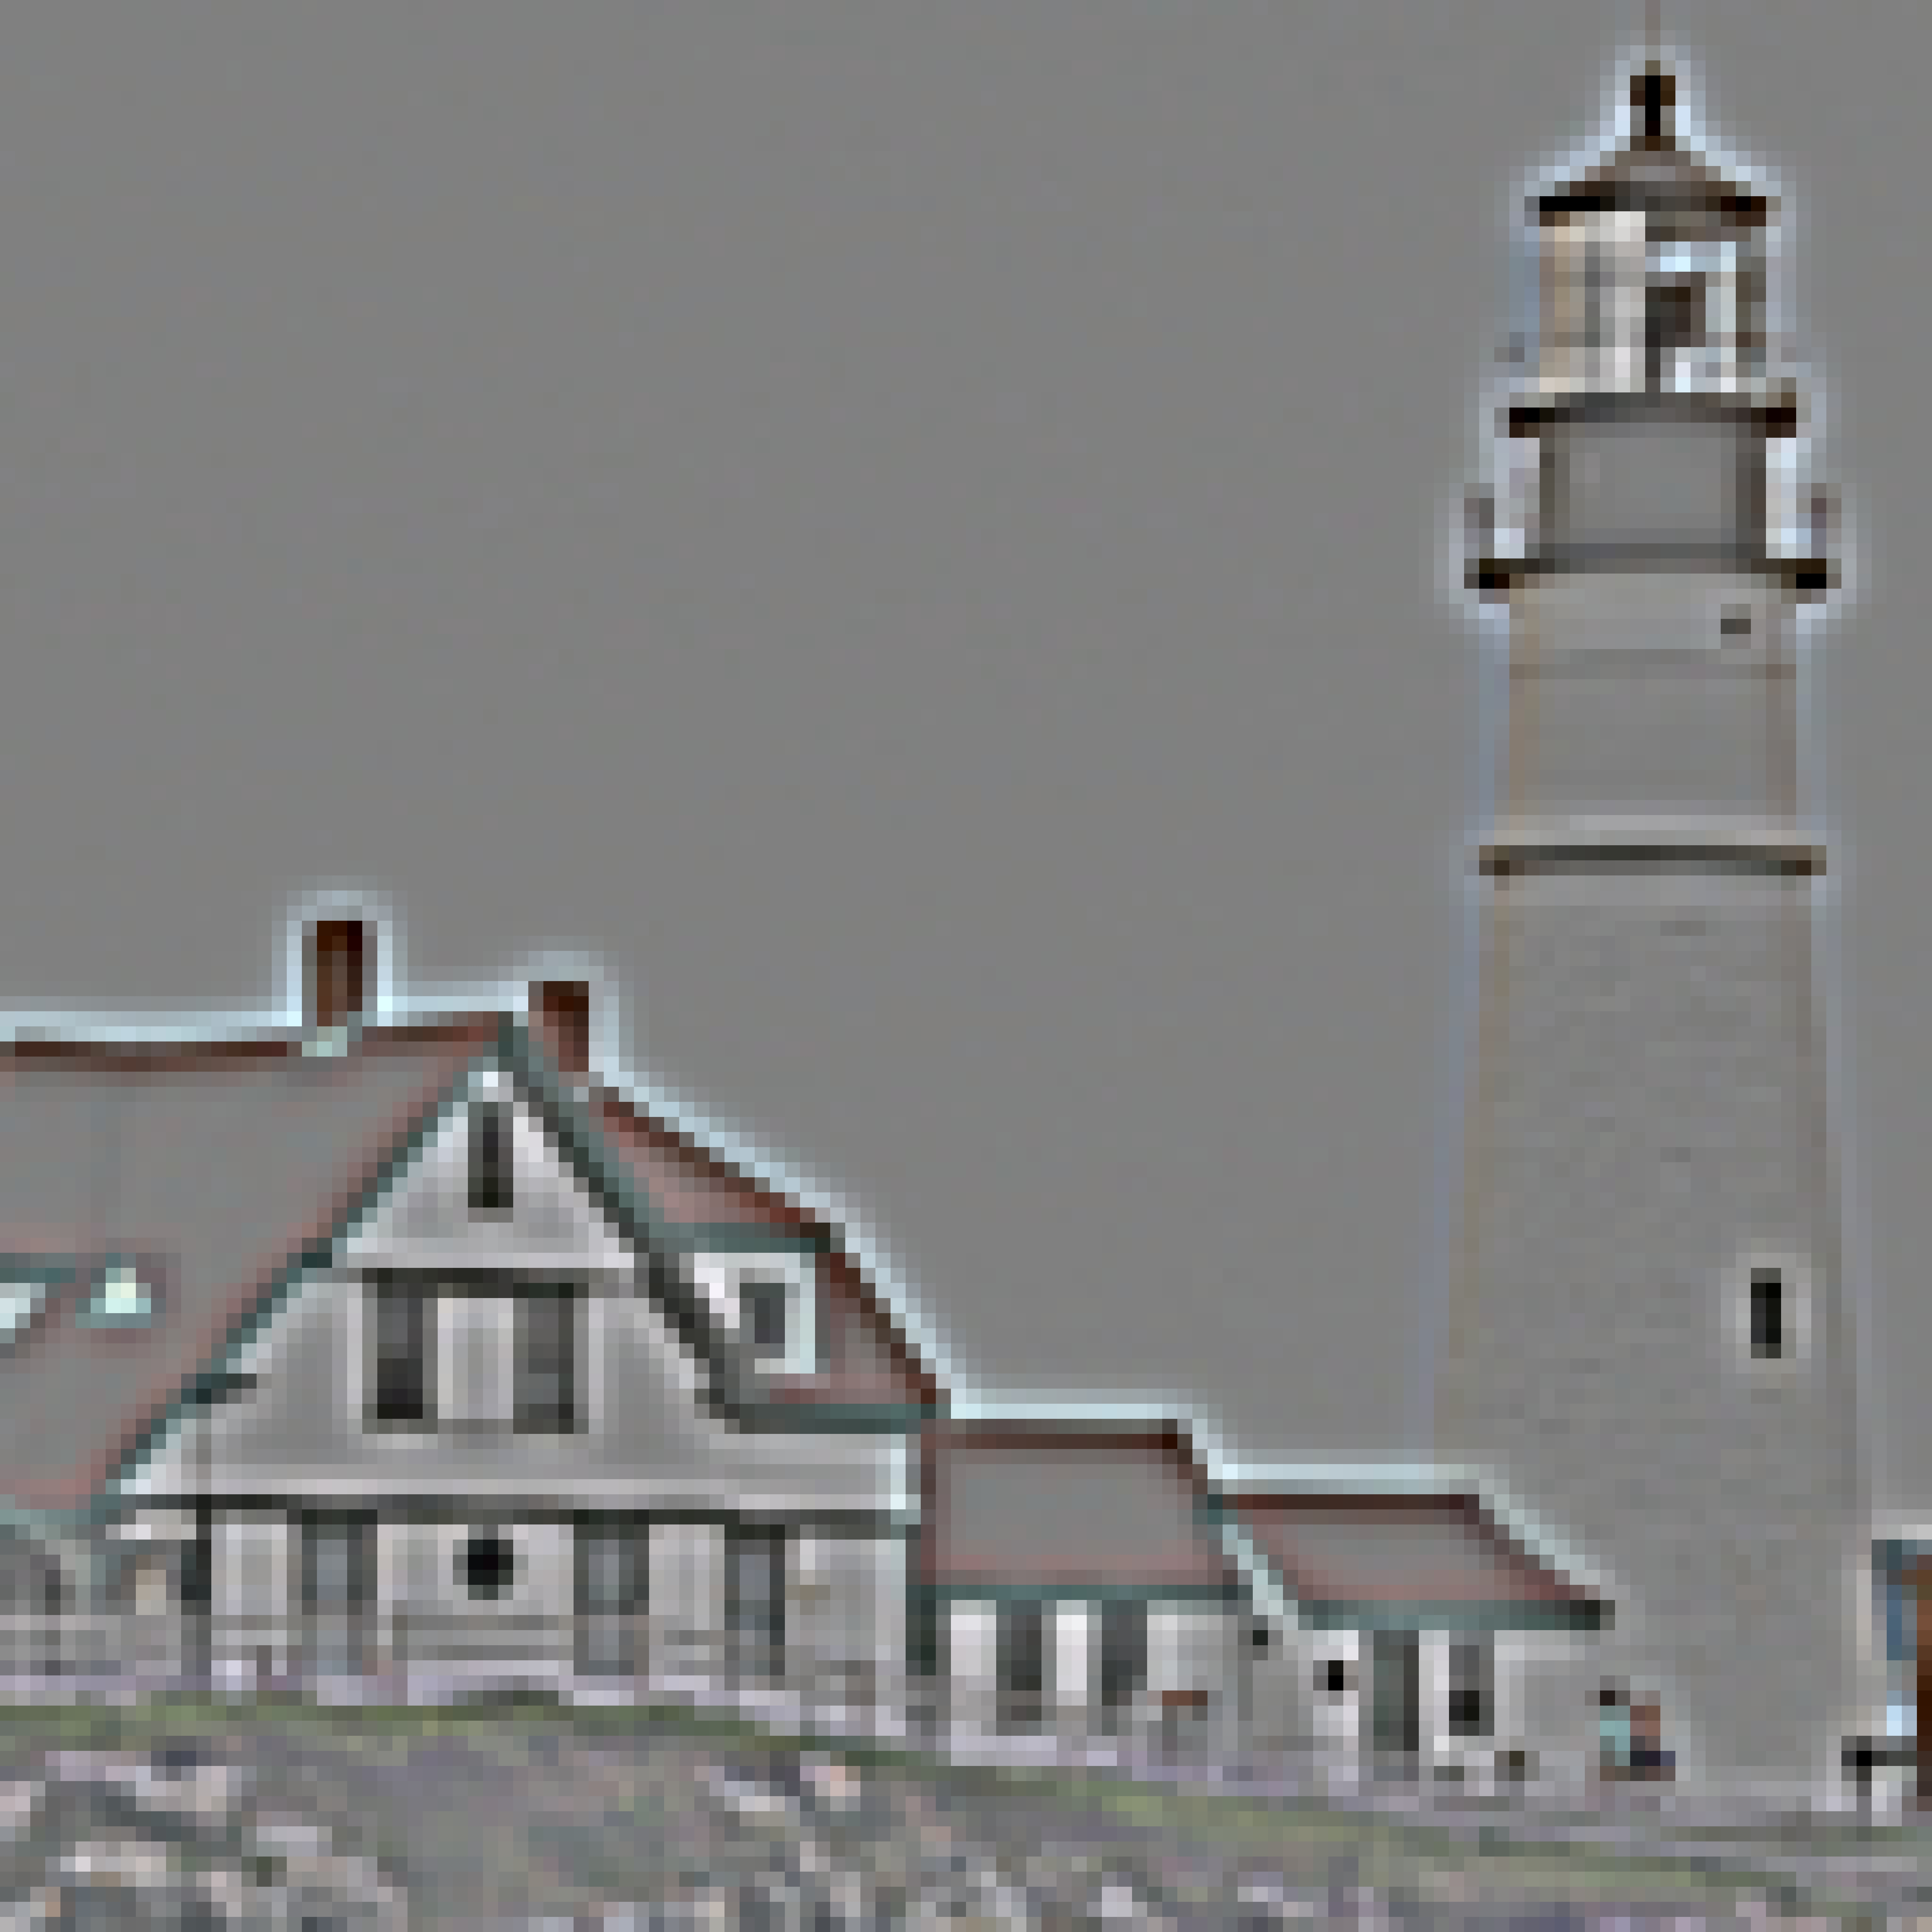
\includegraphics[width=0.25\linewidth]{figures/pyramids/laplacianPyr_2.jpg}
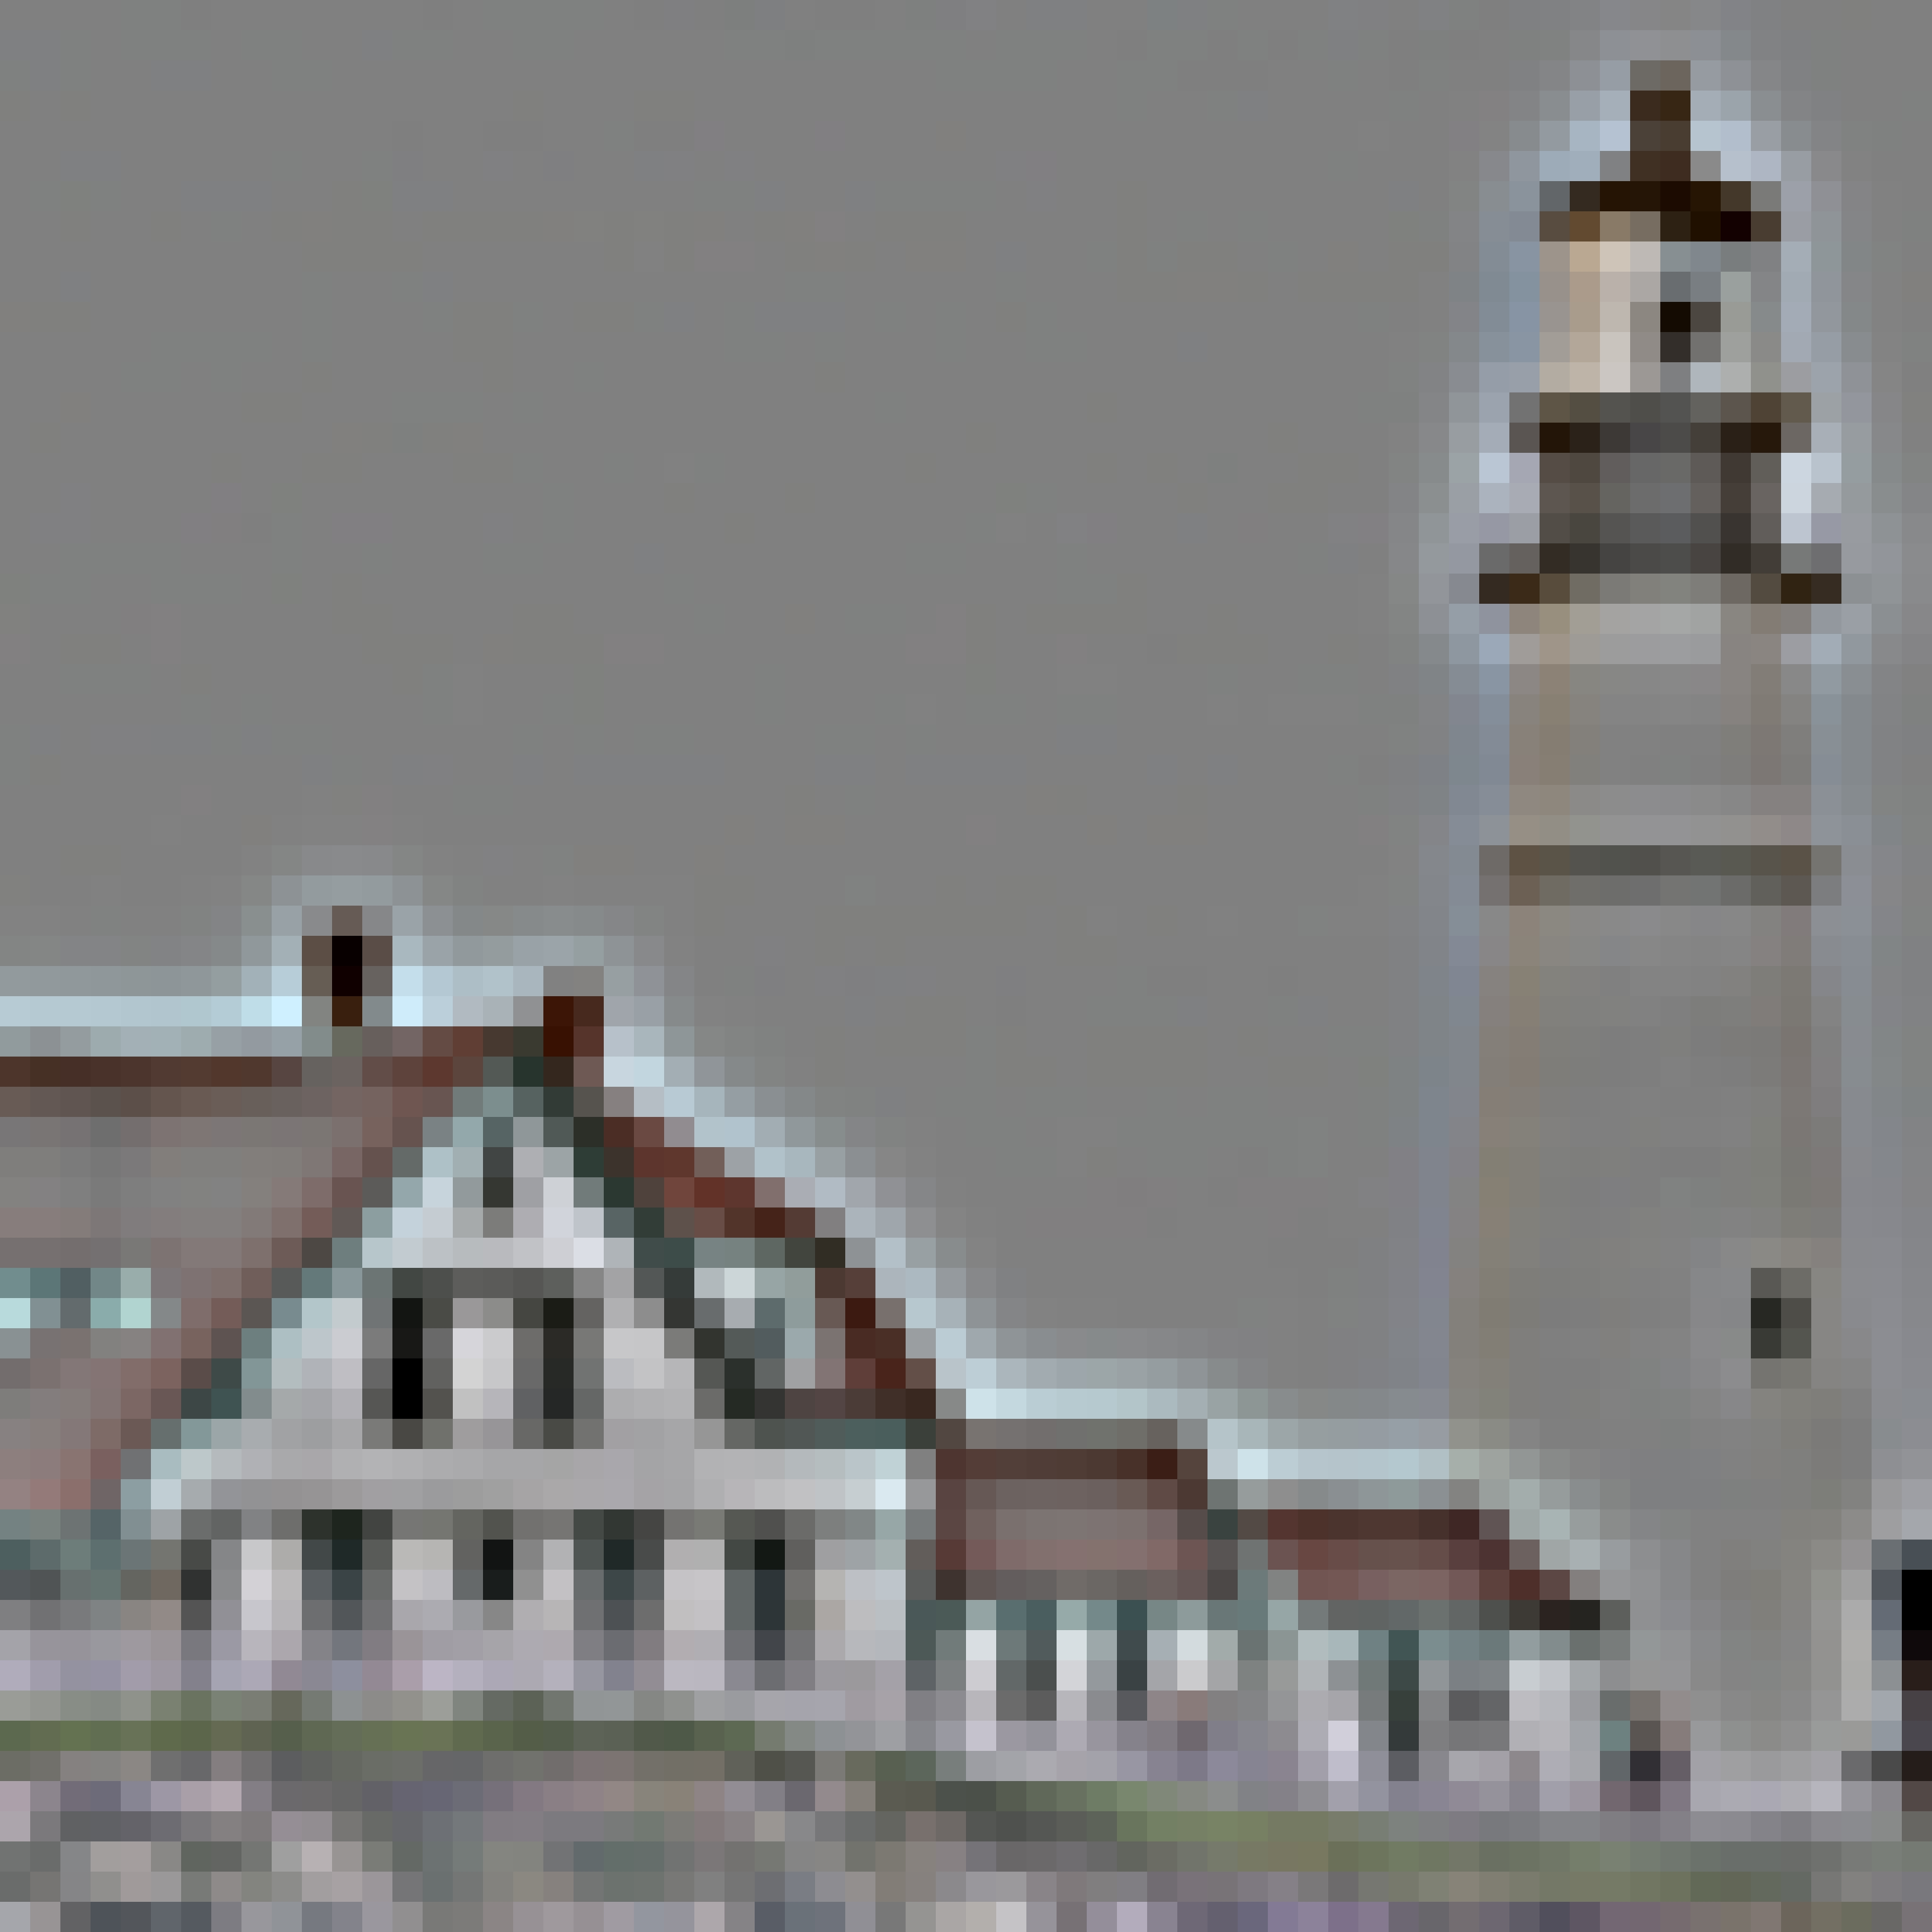
\includegraphics[width=0.125\linewidth]{figures/pyramids/laplacianPyr_3.jpg}
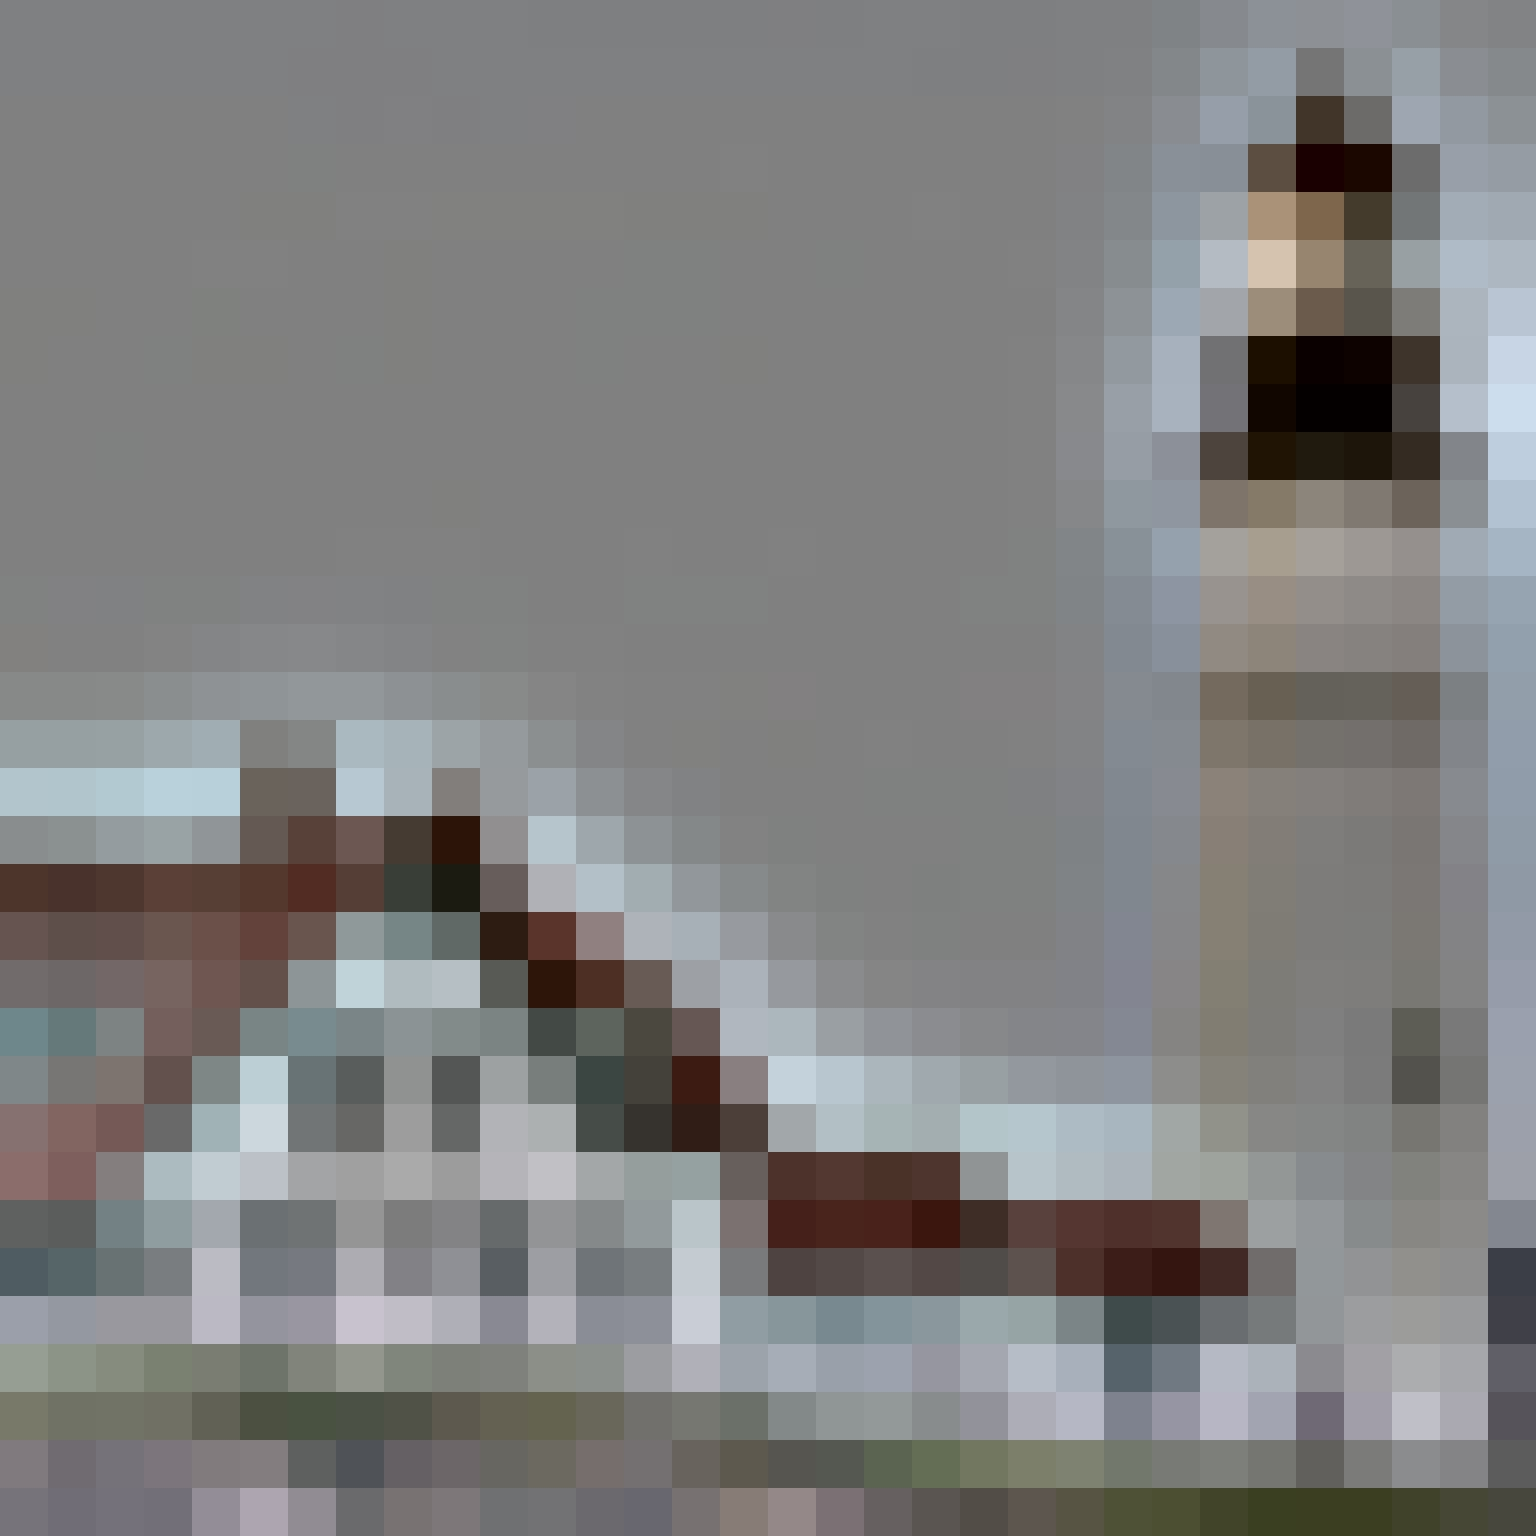
\includegraphics[width=0.0625\linewidth]{figures/pyramids/laplacianPyr_4.jpg}
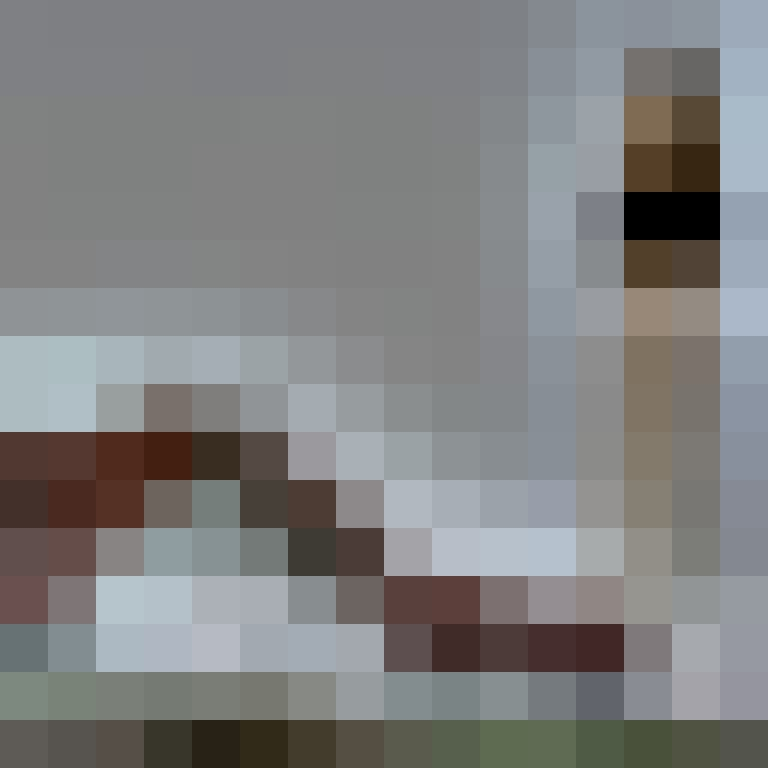
\includegraphics[width=0.03125\linewidth]{figures/pyramids/laplacianPyr_5.jpg}

\includegraphics[width=0.015625\linewidth]{figures/pyramids/gaussianPyr_6.jpg}
}
\caption{Laplacian pyramid, including the low-res residual as the last image.  The Laplacian pyramid is built for each color channel independently.  For visualization, we add 128 to all the images. Therefore, the average gray level corresponds to the zero intensity value.}
\label{fig:gausspyr}
\end{figure}



Interestingly, the Laplacian pyramid is an invertible transform.  We can reconstruct the original image from the Laplacian Pyramid. Using the low-pass residual signal associated with the Laplacian
pyramid, we can recursively reconstruct the corresponding Gaussian pyramid.  Remember that Gaussian pyramid level 1 is just the original image itself, so we can use this to reconstruct the original image
from the Laplacian pyramid, with its lowpass residual:
\begin{equation}
g_k = l_k + F_k g_{k+1}
\label{eq:laplaceRecursion}
\end{equation}

The following diagram contains the Gaussian pyramid, the Laplacian pyramid and the Laplacian inversion for a 3 level Laplacian pyramid. The reconstruction uses the Laplacian pyramid $l_0,l_1,...,l_2$ and the low pass residual $g_3$ to recover the input signal $x=g_0$.

% Definition of blocks:
\tikzset{
  block/.style    = {draw, thin, rectangle, minimum height = 1.5em,  minimum width = 1.5em},
  sum/.style      = {draw, circle, minimum size=.4cm}, % Adder
  input/.style    = {coordinate}, % Input
  output/.style   = {coordinate} % Output
  %x/.style   = {coordinate} % Output
}

\begin{tikzpicture}[auto, thin, node distance=.9cm, >=triangle 45]
% Drawing the blocks of first level:
\draw
	node [input] (x0) {}
	node [right of=x0, node distance=0.5cm] (x0p) {$g_0$}
	%node [input] (x0p) {$x_0$}
	node [block, right of=x0p] (g0) {$G_0$}
         node [block, red, below of=g0] (f0) {$F_0$}
	node [sum, red, left of=f0] (suma0) {}
	node [right of=g0] (x1) {$g_1$}
	node [red, below of=suma0, node distance=2cm] (l0) {$l_0$};
       % Joining blocks. 
	\draw[-](x0) -- node {} (x0p);
	\draw[->](x0p) -- node {} (g0);
	\draw[->,red](x0p) -- node[pos=0.99, left] {{\tiny $+$}} (suma0);
	\draw[->,red](f0) -- node[pos=0.99, below] {{\tiny $-$}} (suma0);
	\draw[->,red](x1) |- node {} (f0);
	\draw[-](g0) |- node {} (x1);
	\draw[->,red](suma0) -- node {} (l0);

\draw
	node [input,right of=x1, node distance=.8cm] (x1p) {}
	%node [input] (x0p) {$x_0$}
	node [block, right of=x1p] (g1) {$G_1$}
        node [block, red, below of=g1] (f1) {$F_1$}
	node [sum, red, left of=f1] (suma1) {}
	node [right of=g1] (x2) {$g_2$}
	node [red, below of=suma1, node distance=1.5cm] (l1) {$l_1$};
       % Joining blocks. 
	\draw[-](x1) -- node {} (x1p);
	\draw[->](x1p) -- node {} (g1);
	\draw[->,red](x1p) -- node[pos=0.99, left] {{\tiny $+$}} (suma1);
	\draw[->,red](f1) -- node[pos=0.99, below] {{\tiny $-$}} (suma1);
	\draw[->,red](x2) |- node {} (f1);
	\draw[-](g1) |- node {} (x2);
	\draw[->,red](suma1) -- node {} (l1);
	
\draw
	node [input,right of=x2, node distance=.8cm] (x2p) {}
	node [block, right of=x2p] (g2) {$G_2$}
        node [block, red, below of=g2] (f2) {$F_2$}
	node [sum, red, left of=f2] (suma2) {}
	node [right of=g2] (x3) {$g_3$}
	node [red, below of=suma2, node distance=1cm] (l2) {$l_2$};
       % Joining blocks. 
	\draw[-](x2) -- node {} (x2p);
	\draw[->](x2p) -- node {} (g2);
	\draw[->,red](x2p) -- node[pos=0.99, left] {{\tiny $+$}} (suma2);
	\draw[->,red](f2) -- node[pos=0.99, below] {{\tiny $-$}} (suma2);
	\draw[->,red](x3) |- node {} (f2);
	\draw[-](g2) |- node {} (x3);
	\draw[->,red](suma2) -- node {} (l2);

\draw
	node [block, blue, right of=x3] (f4) {$F_2$}
	node [sum, blue, right of=f4] (suma4) {{\tiny $+$}}
	node [block, blue, right of=suma4] (f5) {$F_1$}
	node [sum, blue, right of=f5] (suma5) {{\tiny $+$}}
	node [block, blue, right of=suma5] (f6) {$F_0$}
	node [sum, blue, right of=f6] (suma6) {{\tiny $+$}}
	node [input, blue, right of=suma6] (rx) {};
	\draw[->,blue](x3) -- node {} (f4);
	\draw[->,blue](f4) -- node {} (suma4);
	\draw[->,blue](suma4) -- node {} (f5);
	\draw[->,blue](f5) -- node {} (suma5);
	\draw[->,blue](suma5) -- node {} (f6);
	\draw[->,blue](f6) -- node {} (suma6);
	\draw[->,blue](suma6) -- node {} (rx);
	
% reconstruction arrows
	\draw[->,blue](l0) -| node {} (suma6);
	\draw[->,blue](l1) -| node {} (suma5);
	\draw[->,blue](l2) -| node {} (suma4);
\end{tikzpicture}
This architecture has two parts: 1) the analysis network (or encoder) that transforms the input image $x$ into a representation composed of $l_0, l_1, ...$ and the low pass residual $x_n$. And 2) the synthesis network (or decoder) that reconstructs the input from the representation.  The Laplacian pyramid is an overcomplete representation (more coefficients than pixels): the dimensionality of the representation is higher than the dimensionality of the input.

Note that the reconstruction property of the Laplacian pyramid does not depend on the filters used for subsampling and upsampling. Even if we used random filters the reconstruction property would still hold. 

\subsection{Image blending}

The Laplacian pyramid is used in many image processing or analysis applications.  Here we show one fun application:  image blending. The goal is to combine two images into one. A mask is used to define how the images will be combined. If we want to blend the following two images using the mask shown in the right:
\begin{figure}[h!]
\centerline{
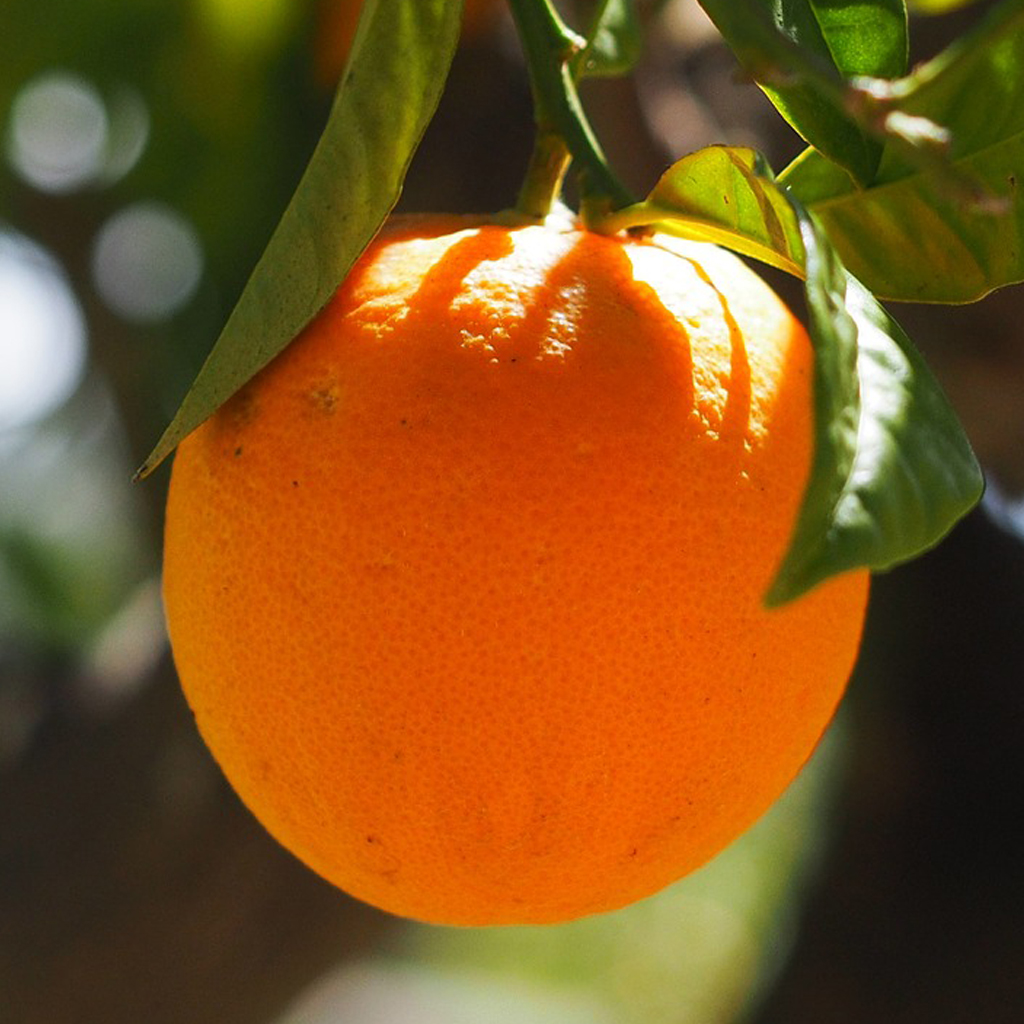
\includegraphics[width=0.20\linewidth]{figures/pyramids/orange.jpg}
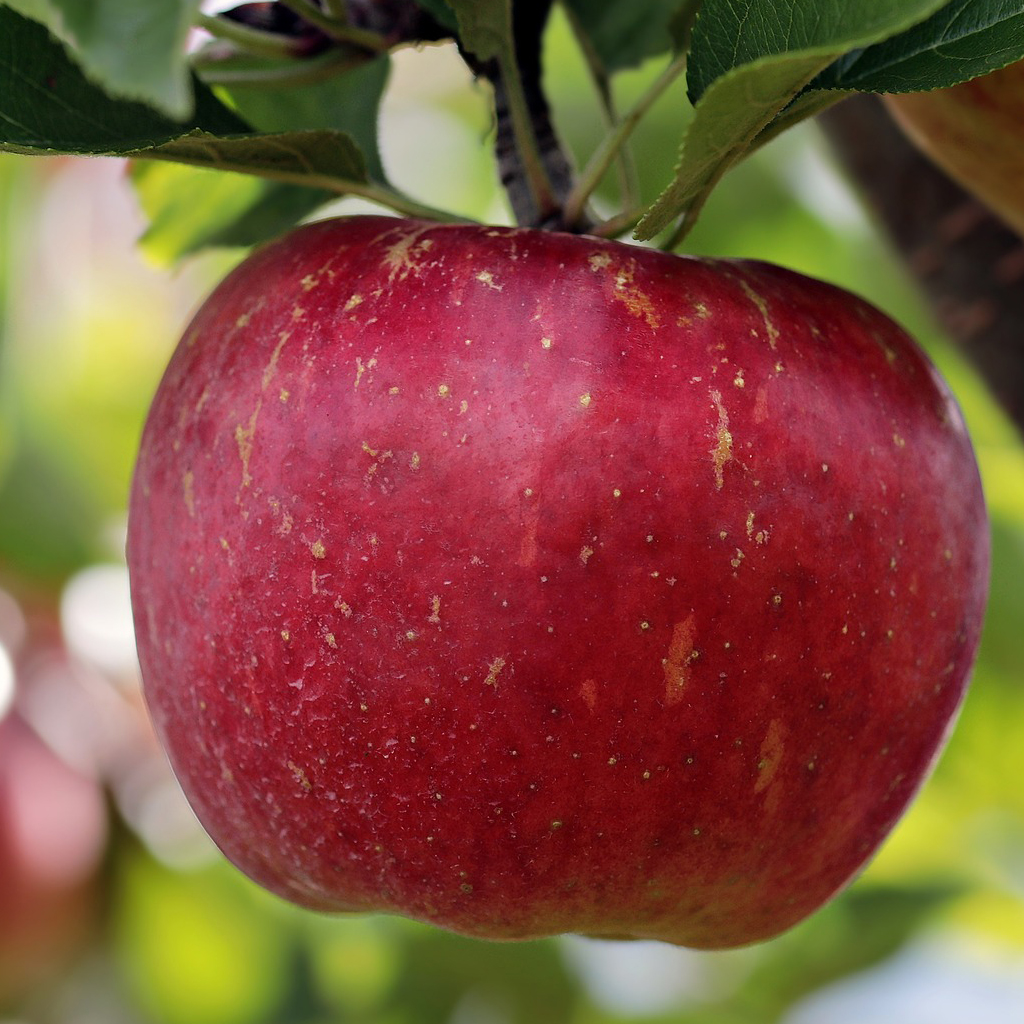
\includegraphics[width=0.20\linewidth]{figures/pyramids/apple.jpg}

\includegraphics[width=0.20\linewidth]{figures/pyramids/mask10.jpg}
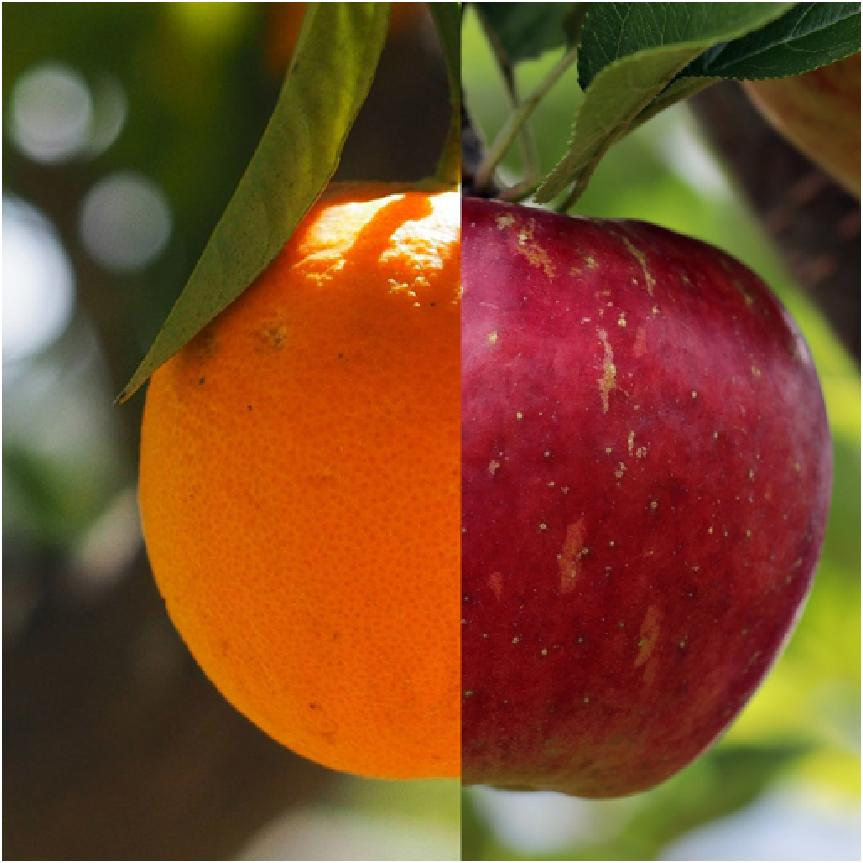
\includegraphics[width=0.20\linewidth]{figures/pyramids/apple_orange_mask_8levels.jpg}
}
\end{figure}
%The Laplacian pyramid is used in many image processing or analysis
%applications.  Here we show one fun application:  image blending
%(you'll do this in a homework problem).  

Making a sharp transition from one image to another gives an artifactually sharp image boundary (see the straight edge of the apple/orange.)

% Tedfest, Burt's talk. 

Using the Laplacian pyramid, we can transition from one image to the next over many different spatial scales to make a gradual transition between the two images. First, we build the Laplacian pyramid for the two input images, in this example we use 7 levels and we also keep the last low-pass residual:
\begin{figure}[h!]
\centerline{
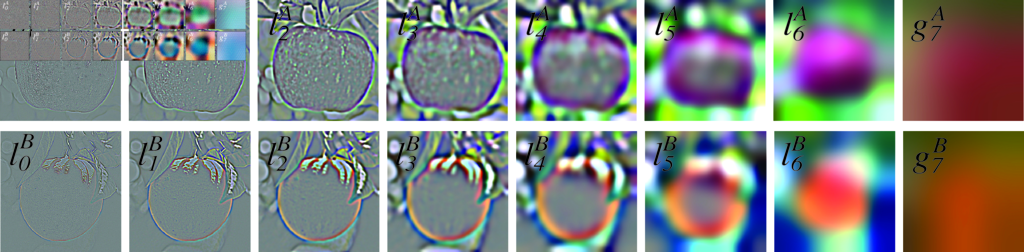
\includegraphics[width=0.9\linewidth]{figures/pyramids/blending_pyrs.eps}
}
\end{figure}

and the Gaussian pyramid of the mask as shown below (note that we use 8 levels, one level more than for the Laplacian pyramid):
\begin{figure}[h!]
\centerline{
\includegraphics[width=0.9\linewidth]{figures/pyramids/blending_pyrs_mask.eps}
}
\end{figure}

%as shown in the apple/orange in the bottom right of Fig.~\ref{fig:appleorange}. 
%To do this, both images are analyzed first by the Laplacian pyramid. The mask is analyzed by the Gaussian pyramid. 
Now we combine the three pyramids to compute the Laplacian pyramid of the blended image. The Laplacian pyramid of the blended image is obtained as: $l_k = l_k^A * m_k + l_i^B * (1-m_k)$. The same is done for the low-pass residual. 

\begin{figure}[h!]
%\centerline{
%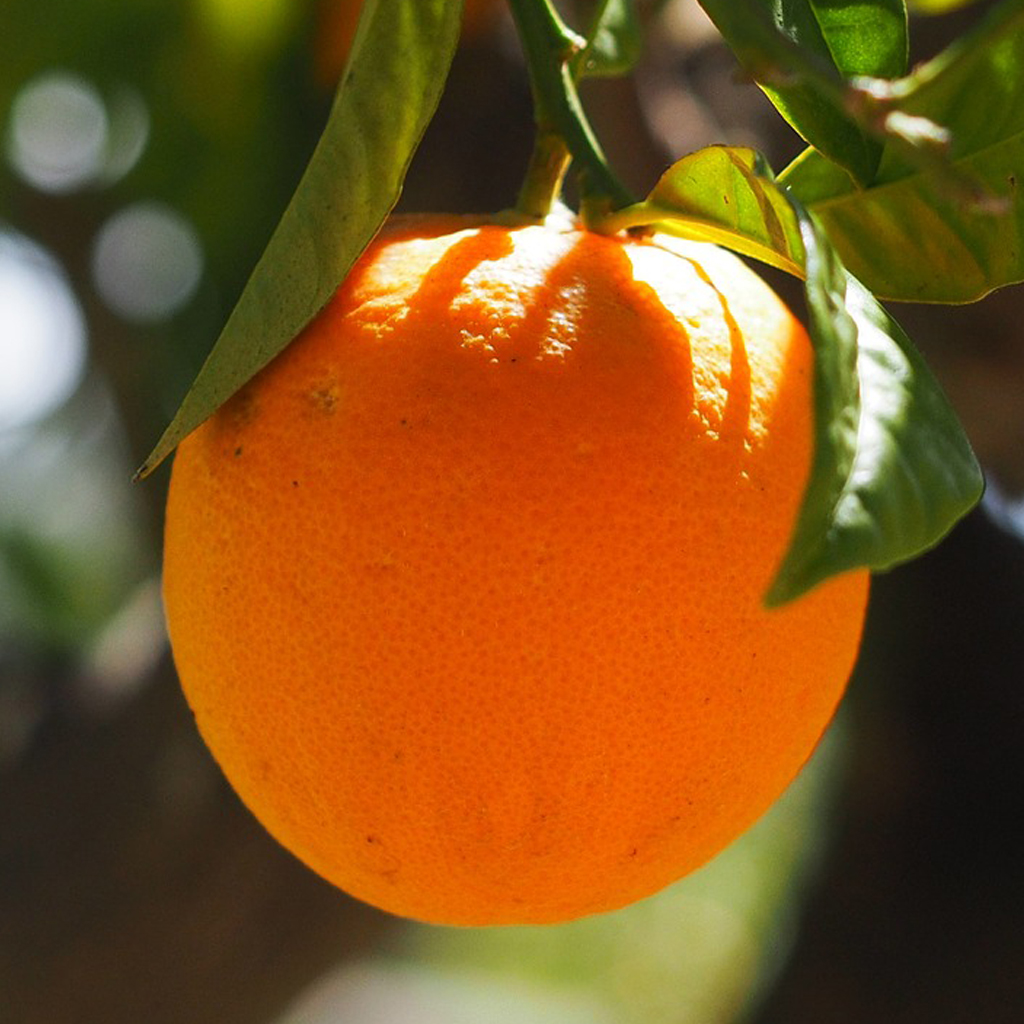
\includegraphics[width=0.3\linewidth]{figures/pyramids/orange.jpg}
%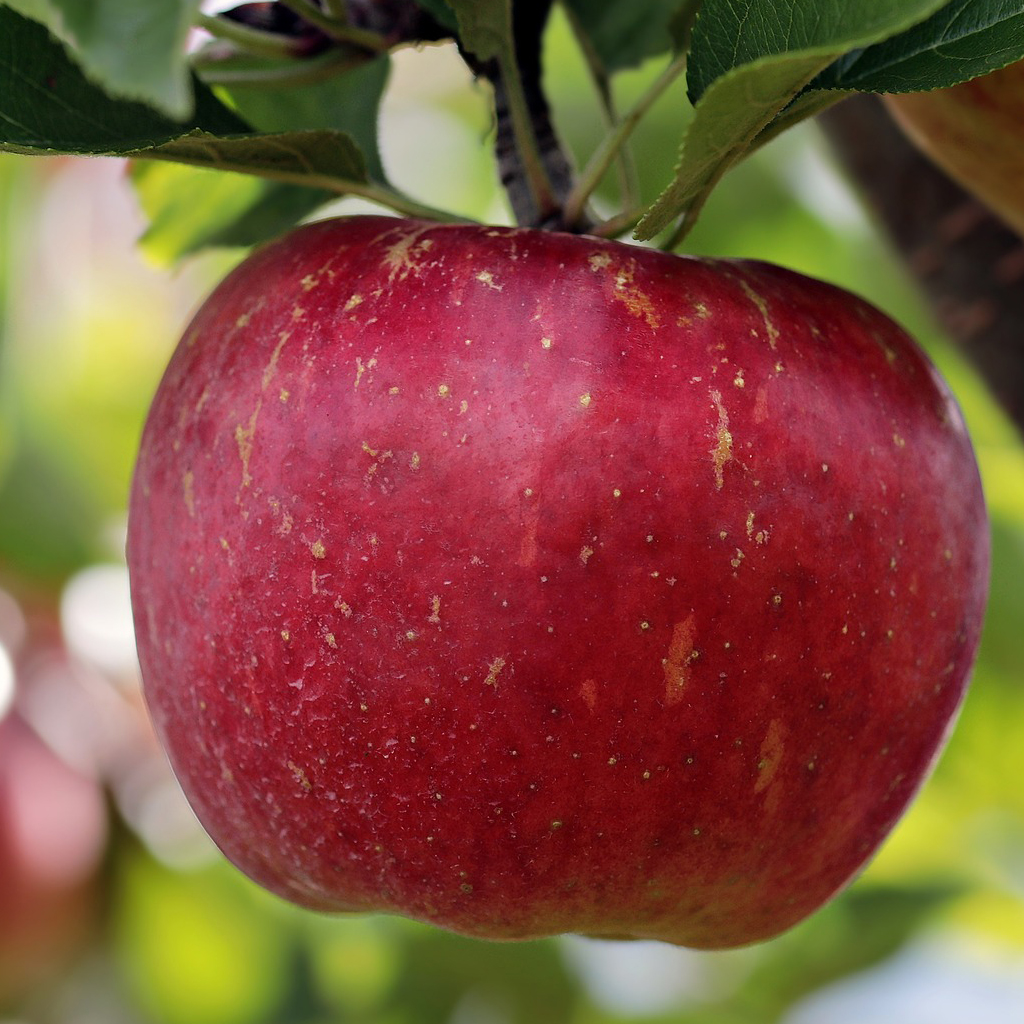
\includegraphics[width=0.3\linewidth]{figures/pyramids/apple.jpg}
%
\includegraphics[width=0.3\linewidth]{figures/pyramids/mask10.jpg}
%}
%\centerline{
%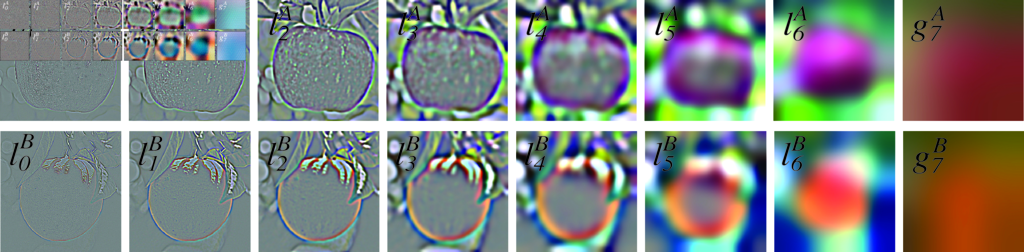
\includegraphics[width=0.9\linewidth]{figures/pyramids/blending_pyrs.eps}
%}
\centerline{
%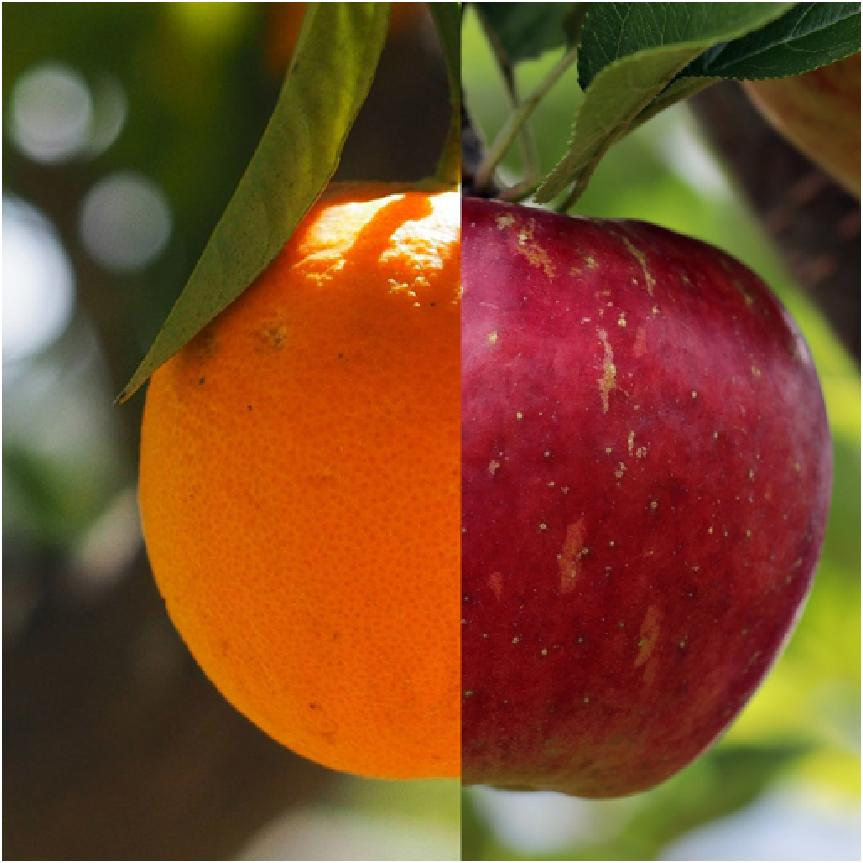
\includegraphics[width=0.45\linewidth]{figures/pyramids/apple_orange_mask_8levels.jpg}
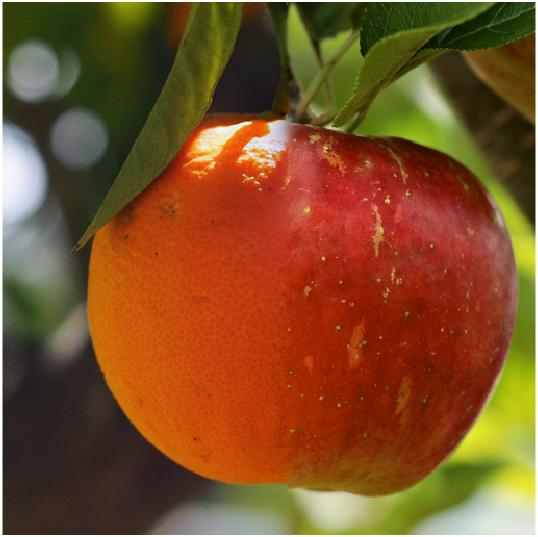
\includegraphics[width=0.45\linewidth]{figures/pyramids/apple_orange_laplacian_8levels.jpg}
}
%\caption{image compositing example.}
\label{fig:appleorange}
\end{figure}
%
%


%


%
%
%\begin{figure}
%\centerline{
%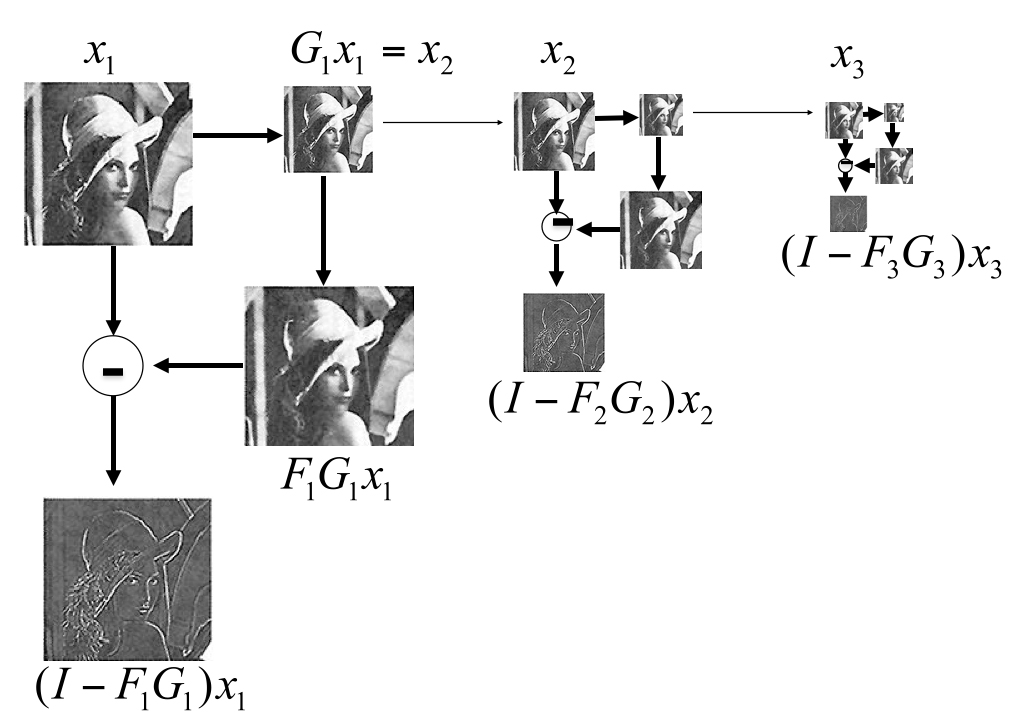
\includegraphics[width=0.5\linewidth]{figures/pyramids/lmat.jpg}
%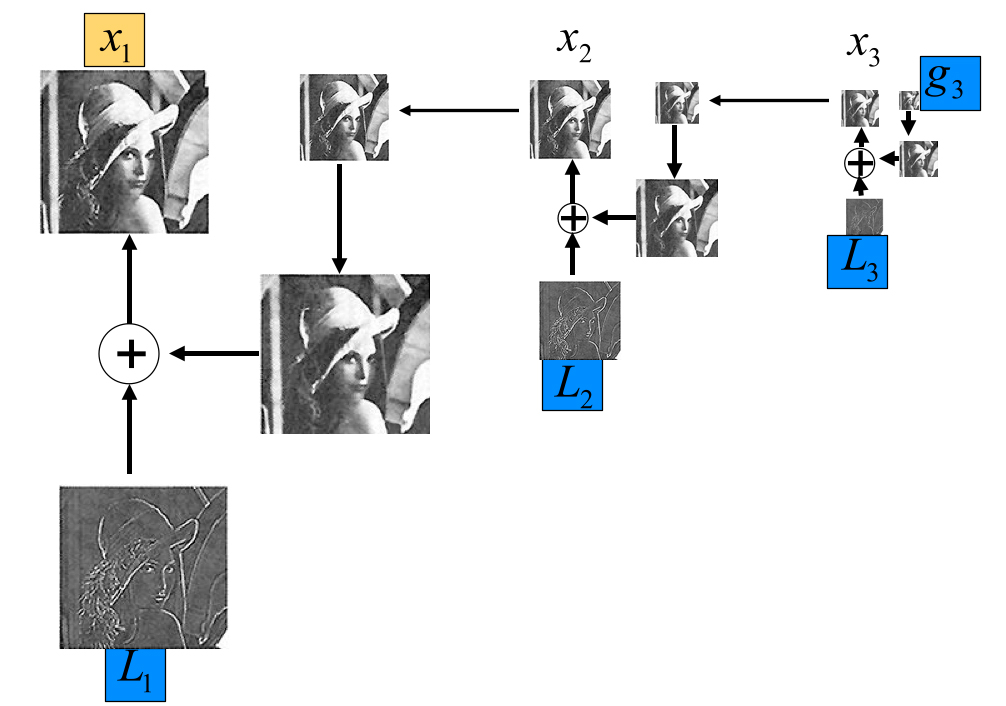
\includegraphics[width=0.5\linewidth]{figures/pyramids/lmatrecon.jpg}
%}
%\caption{Laplacian pyramid construction, and reconstruction from that
%  representation. }
%\label{fig:lmat}
%\end{figure}
%
%
%The Laplacian pyramid is simple:  it represents, at each level, what
%is present in a Gaussian pyramid image of one level, but not present
%at the level below it.  We calculate that by expanding the
%lower-resolution Gaussian pyramid image to the same pixel resolution
%as the neighboring higher-resolution Gaussian pyramid image, then
%subtracting the two.  This calculation is made in a recursive,
%telescoping fashion.  By storing a recursion-ending Gaussian
%low-resolution image, the original image can be reconstructed from its
%Laplacian pyramid representation, Fig.~\ref{fig:lmat}.
%
%
%\begin{figure}
%\centerline{
%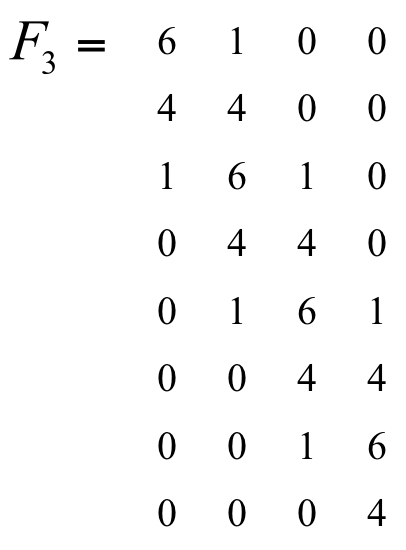
\includegraphics[width=0.2\linewidth]{figures/pyramids/upsamp.jpg}
%}
%\caption{The blur-and-upsample operator, shown for a 1-d signal.  A 2-d
%  implementation can be achieved with the 1-d version applied
%  separably in each dimension. }
%\label{fig:upsamp}
%\end{figure}
%
%%\subsubsection{Laplacian pyramid steps}
%
%Here are the steps for calculating a Laplacian pyramid.  Let the
%operator $G_n$ be the blur-and-downsample operator at pyramid level $n$.
%This is shown in Fig.~\ref{fig:gpnums}.  Let $F_n$ be the
%blur-and-upsample operator for pyramid level $n$, shown in
%Fig.~\ref{fig:upsamp}.   Then the Laplacian pyramid coefficients,
%$L_n$, at pyramid level $n$, are:  
%\begin{equation}
%L_n = (I_n - F_n G_n) x_n,
%\end{equation}
%where $I_n$ is the identity operator for pyramid level $n$, and $x_n$
%is the Gaussian pyramid coefficients for the image at level $n$.
%
%Using the low-pass residual signal associated with the Laplacian
%pyramid, we can recursively reconstruct the corresponding Gaussian
%pyramid.  Remember that Gaussian pyramid level 1 is just the original
%image itself, so we can use this to reconstruct the original image
%from the Laplacian pyramid, with its lowpass residual:
%\begin{equation}
%x_n = L_n + F_n x_{n+1}
%\label{eq:laplaceRecursion}
%\end{equation}
%A repeated applications of Eq.~(\ref{eq:laplaceRecursion}), we can
%recover $x_1$, the original image.
%
%
%\begin{figure}
%\centerline{
%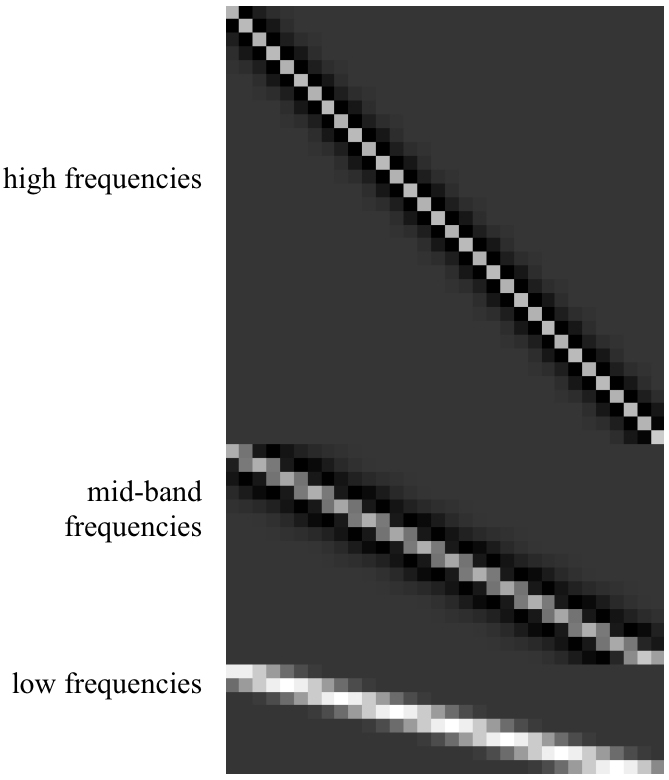
\includegraphics[width=0.4\linewidth]{figures/pyramids/lapmat.jpg}
%}
%\caption{Matrix visualization of Laplacian pyramid. }
%\label{fig:lapmat}
%\end{figure}
%
%Fig.~\ref{fig:lapmat}
% is the equivalent matrix which creates a 1-d Laplacian pyramid
%from an input column vector (again, the actual computation is more
%efficient than is multiplying by this matrix).
%
%\begin{figure}
%\centerline{
%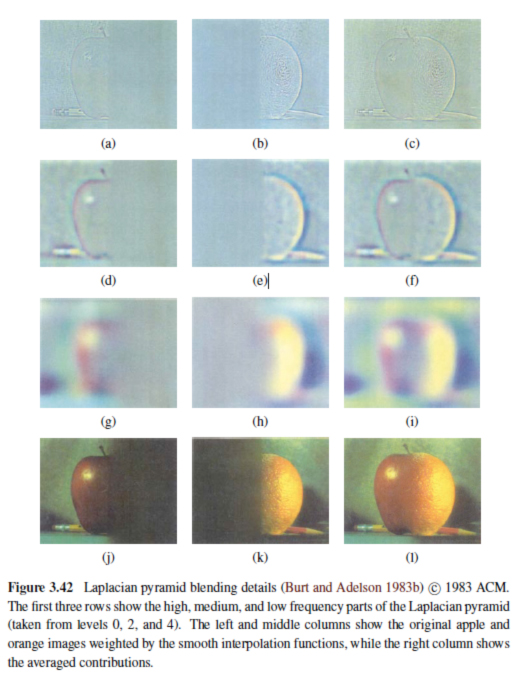
\includegraphics[width=0.55\linewidth]{figures/pyramids/appleLaplace.jpg}
%}
%\caption{Laplacian pyramid for image compositing}
%\label{fig:appleLaplace}
%\end{figure}
%
%
%\subsection{Haar and QMF pyramids}
%
%\subsubsection{1-d Haar transform}
%
%The Laplacian pyramid is an overcomplete representation (more
%coefficients than pixels).  The wavelet (or sometimes called a
%quadrature mirror filter (QMF) pyramid, in the signal processing
%community) transform will be complete (instead of overcomplete), and
%adds some orientation tuning.  The Haar transform is the simplest
%version, yet still has many of the properties of other wavelet
%transforms, so let's derive that first.
%
%Suppose we have the submatrix, U.   The first coefficient of the
%transform is just the average of the two input pixels, and the 2nd
%coefficient it the difference.  Clearly, that's an invertible change
%of basis, and the inverse is shown here as $U^{-1}$.  
%
%
%\begin{figure}
%\centerline{
%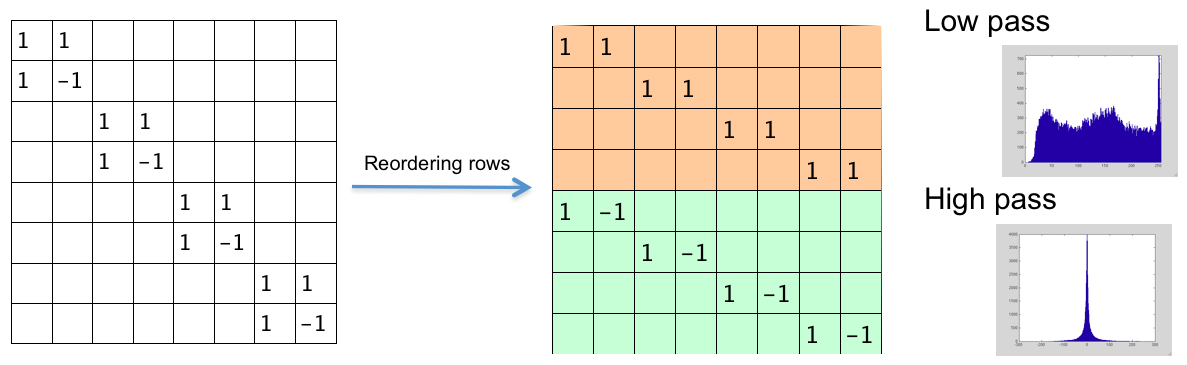
\includegraphics[width=0.7\linewidth]{figures/pyramids/haar1.jpg}
%}
%\centerline{
%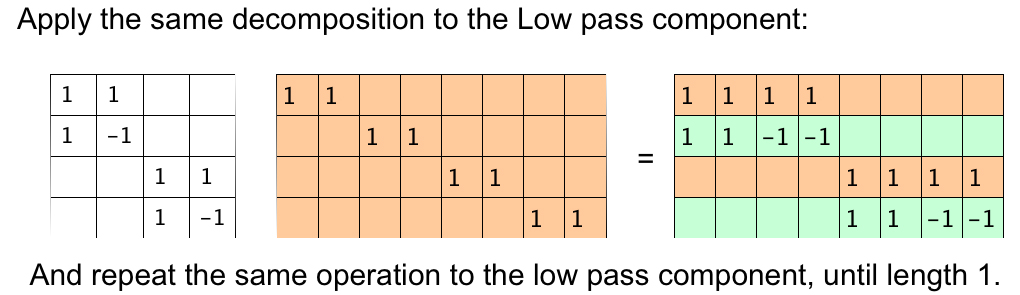
\includegraphics[width=0.7\linewidth]{figures/pyramids/haar2.jpg}
%}
%\caption{Haar wavelet decomposition}
%\label{fig:haar1d1}
%\end{figure}
%
%
%
%
%One thing to note here is the aliasing of each subband,
%and its cancellation when the two subbands are combined.   In both the
%high and the low bands, we're taking every other sample of a signal
%convolved with some two-tap filter.  Those two-tap (high or low-pass)
%filters don't sufficiently pre-filter the signal to avoid aliasing in
%the resulting subsampled signal.  So how do we obtain perfect
%reconstruction from those filter banks?  Each band relies on the other
%one to supply the information needed to removing the aliasing that
%happens from one band alone.  (We can easily see how the other band is
%used for reconstruction in the space-domain view of things.  The
%Fourier domain explanation involves the aliasing components from each band
%that cancel each other.)
%
%We can replicate this submatrix in different subspaces of a larger
%matrix, and re-order the rows to make it obvious that we're creating a
%low-pass version of the signal, and a high-pass one.
%Fig.~\ref{fig:haar1d2} shows another construction of the Haar transform
%matrix, and its inverse.
%
%
%\begin{figure}
%\centerline{
%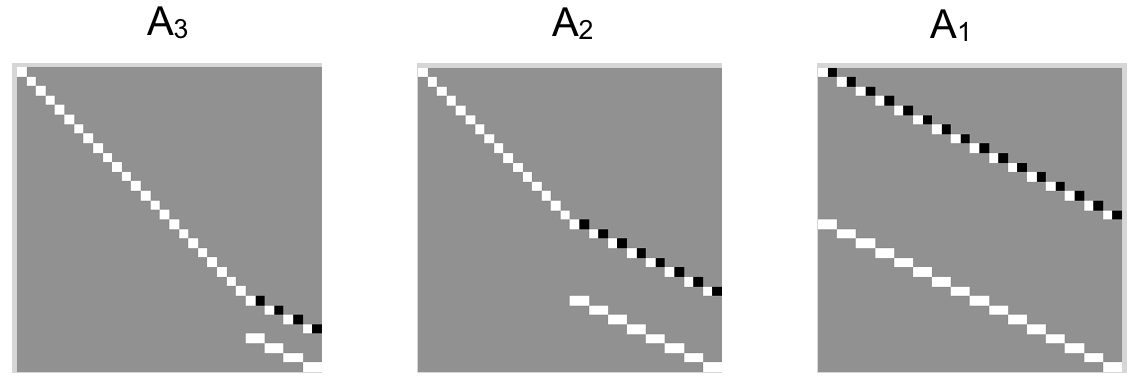
\includegraphics[width=0.7\linewidth]{figures/pyramids/haar3.jpg}
%}
%\centerline{
%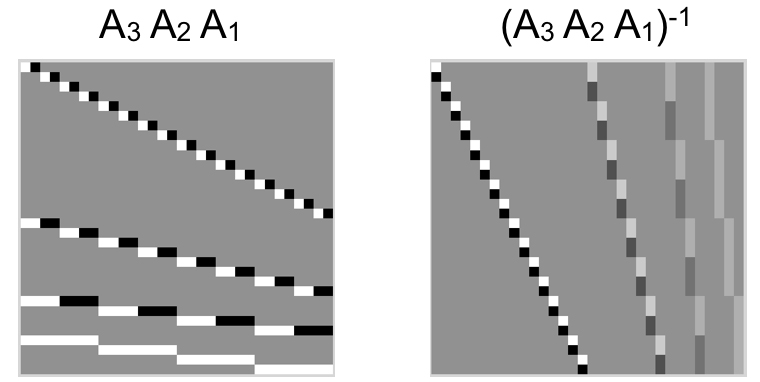
\includegraphics[width=0.5\linewidth]{figures/pyramids/haar4.jpg}
%}
%\caption{more on 1-d haar wavelet}
%\label{fig:haar1d2}
%\end{figure}
%
%\subsubsection{2-d Haar transform}
%
%We apply the 1-d Haar transform separably in 2-d, which leads to:  a
%low-pass band, a vertical high-pass band, a horizontal high-pass band,
%and a ``diagonal'' band, high-pass in both horizontal and vertical.
%Unfortunately, that last band isn't a rotation of either of the other
%two band-pass bands.    The wavelet transform is great for
%compression, since it's ``complete'', with the same number of
%coefficients as pixels.  For the Haar filter, reconstruction from the
%transform domain is exact, but for other filters it is only
%approximate.
%
%The Haar filters are just the simplest
%example of an orthonormal wavelet, or QMF, filter set.  Larger filters
%have only approximate image reconstruction, but have nicer frequency
%localization properties and are generally used instead of the Haar filters.
%
%\begin{figure}
%\centerline{
%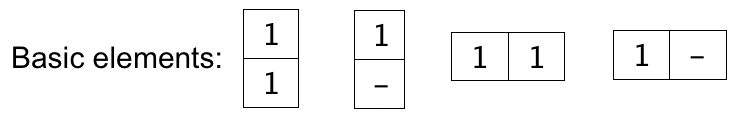
\includegraphics[width=0.4\linewidth]{figures/pyramids/haar2d1.jpg}
%}
%\centerline{
%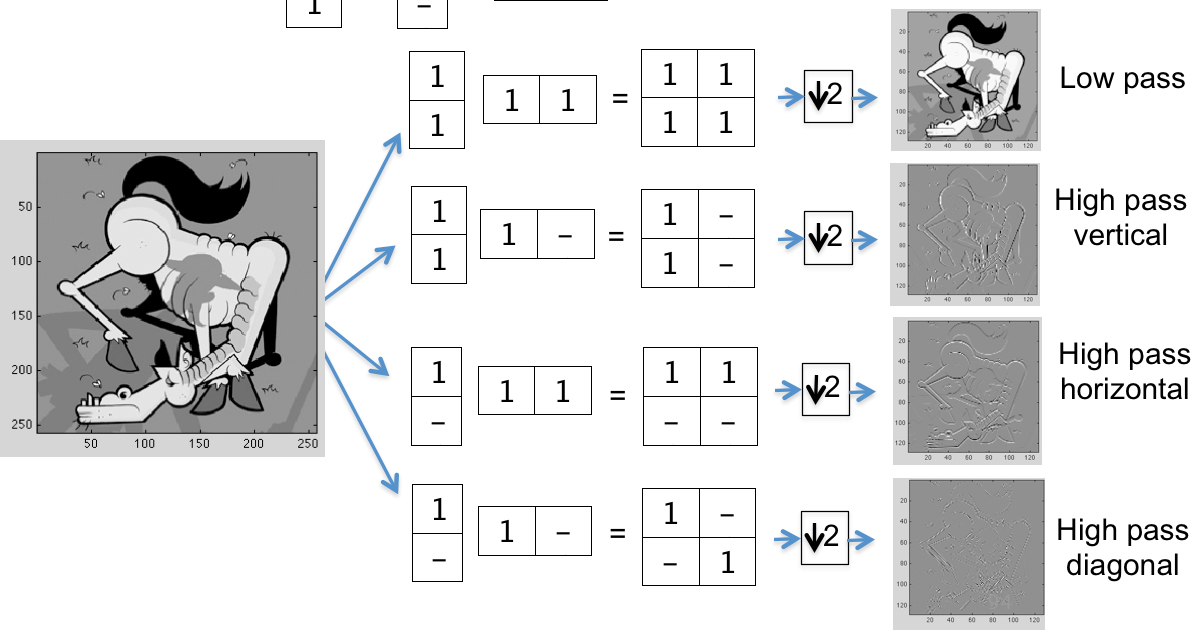
\includegraphics[width=0.8\linewidth]{figures/pyramids/haar2d2.jpg}
%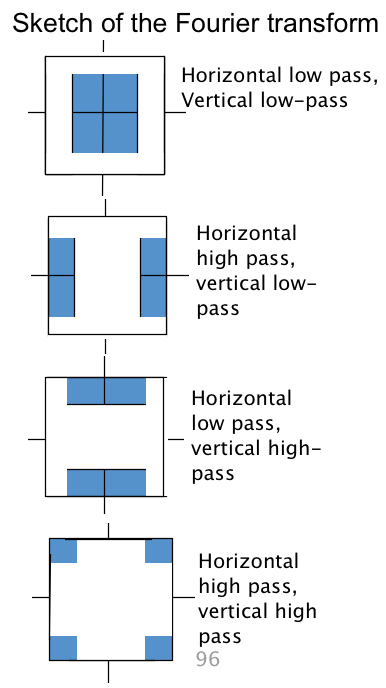
\includegraphics[width=0.24\linewidth]{figures/pyramids/haar2d3.jpg}
%}
%\caption{2d haar wavelet}
%\label{fig:haar2d}
%\end{figure}
%
%
%
%
%The price we pay for the completeness property is that each subband is
%aliased.  We want each subband, by itself, to tell us something abou
%the image components in a particular frequency band.  But these
%aliased subbands don't tell us such a clean story.  Figure~\ref{fig:splat} is a
%simple demonstration of that.  The top row shows an example signal,
%translated by one pixel from the left column to the right.  the three
%rows below in each column show the wavelet/qmf filter subband
%representation .  (see discussion at slide 88).  At one position of
%the signal, our representation tells us that all the signal energy is
%confined to just one sub-band.  But then we move the signal one pixel
%forward and the signal is represented as a splattering of coefficient
%values across different subbands.  This limits the usefulness of
%complete orthonormal wavelets for various image analysis applications
%(for example, you couldn't compute stereo offsets between two images
%within such a representation).
%
%
%\begin{figure}
%\centerline{
%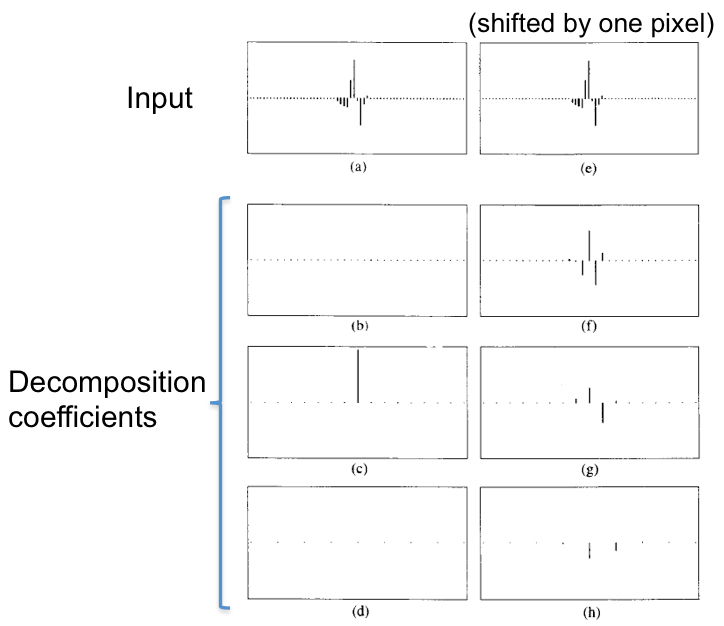
\includegraphics[width=0.6\linewidth]{figures/pyramids/splat.jpg}
%}
%\caption{showing translation variance of an aliased subband representation}
%\label{fig:splat}
%\end{figure}
%
%
%
%
%
\section{Steerable pyramid}
%

The Laplacian pyramid provides a richer representation than the Gaussian pyramid. But we would like to have an even more expressive image representation.  The steerable pyramid adds information about image orientation. Therefore, the Steerable  representation is a multi-scale oriented representation that is translation-invariant. It is non-aliased and self-invertible. Ideally, we'd like to have an image transformation that was
shiftable--where we could perform interpolations in position, scale,
and orientation using linear combinations of a set of basis
coefficients.  The steerable pyramid goes part way there.

\marginnote{One {\bf block} of the Steerable pyramid computation.
\\~\\
%\tikzset{
%  block/.style    = {draw, thin, rectangle, minimum height = 1.5em,  minimum width = 1.5em},
%  sum/.style      = {draw, circle, minimum size=.4cm}, % Adder
%  input/.style    = {coordinate}, % Input
%  output/.style   = {coordinate} % Output
%}
\begin{tikzpicture}[auto, thin, node distance=.8cm, >=triangle 45]
%% Drawing the blocks of first level:
\draw
	node [] (x0) {$g_k$}
	node [input,right of=x0, node distance=0.4cm] (x0p) {}
	node [block, right of=x0p] (b0) {$B_0$}
         node [block, below of=b0] (b1) {$B_1$}
         node [block, below of=b1] (bk) {$B_n$}
         node [block, below of=bk] (L1) {$L$}
         node [block, right of=L1] (D2) {$D$}
         node [right of=b0, node distance=1.1cm] (b0out) {$b_{k,0}$}
         node [right of=b1, node distance=1.1cm] (b1out) {$b_{k,1}$}
         node [right of=bk, node distance=1.1cm] (bkout) {$b_{k,n}$}
         node [right of=D2, node distance=1.1cm] (out) {$g_{k+1}$};
       % Joining blocks. 
	\draw[-](x0) -- node {} (x0p);
	\draw[->](x0p) -- node {} (b0);
	\draw[->](x0p) |- node {} (b1);
	\draw[->](x0p) |- node {} (bk);
	\draw[->](x0p) |- node {} (L1);
	\draw[->](L1) -- node {} (D2);
	\draw[->](b0) -- node {} (b0out);
	\draw[->](b1) -- node {} (b1out);
	\draw[->](bk) -- node {} (bkout);
	\draw[->](D2) -- node {} (out);
\end{tikzpicture}
}

We analyze in orientation using a steerable filter bank.  We form a
decomposition in scale by introducing a low-pass filter (designed to
work with the selected bandpass filters), and recursively breaking the
low-pass filtered component into angular and low-pass frequency
components.   Pyramid subsampling steps are preceded by sufficient
low-pass filtering to remove aliasing.

To ensure that the image can be reconstructed from the steerable
filter transform coefficients, the filters must be designed so that
their sums of squared magnitudes ``tile'' in the frequency domain.  We
reconstruct by applying each filter a second time to the steerable
filter representation, and we want the final system frequency response
to be flat, for perfect reconstruction.

\begin{figure}[h!]
\centerline{
\includegraphics[width=0.80\linewidth]{figures/pyramids/steerable_pyr_sp3Filters.eps}
}
\end{figure}


The following block diagram shows the steps to build a 2 level steerable pyramid and the reconstruction of the input. The architecture has two parts: 1) the analysis network (or encoder) that transforms the input image $x$ into a representation composed of $r=\left[ b_{0,0},...,b_{0,n}, b_{1,0},...b_{1,n},...,b_{k-1,0},...b_{k-1,n} \right]$ and the low pass residual $g_{k-1}$. And 2) the synthesis network (or decoder) that reconstructs the input from the representation $r$.  

% Definition of blocks:
%\tikzset{
%  block/.style    = {draw, thin, rectangle, minimum height = 1.5em,  minimum width = 1.5em},
%  sum/.style      = {draw, circle, minimum size=.4cm}, % Adder
%  input/.style    = {coordinate}, % Input
%  output/.style   = {coordinate} % Output
%  %x/.style   = {coordinate} % Output
%}
%%. DRAWING THE STEERABLE PYRAMID
\begin{tikzpicture}[auto, thin, node distance=.9cm, >=triangle 45]
% Drawing the blocks of first level:
\draw
	node [] (x0) {$x$}
	node [input,right of=x0, node distance=0.5cm] (x0p) {}
	node [block, right of=x0p] (b0) {$B_0$}
         node [block, below of=b0] (b1) {$B_1$}
         node [block, below of=b1] (bk) {$B_n$}
         node [block, below of=bk] (L1) {$L$}
         node [block, right of=L1] (D2) {$D$};
       % Joining blocks. 
	\draw[-](x0) -- node {} (x0p);
	\draw[->](x0p) -- node {} (b0);
	\draw[->](x0p) |- node {} (b1);
	\draw[->](x0p) |- node {} (bk);
	\draw[->](x0p) |- node {} (L1);
	\draw[->](L1) -- node {} (D2);

% Drawing the blocks of second level:
\draw
	%node [input, right of=D2] (x1) {}
	node [input, right of=D2, node distance=0.5cm] (x1p) {}
	node [block, right of=x1p] (b10) {$B_0$}
         node [block, below of=b10] (b11) {$B_1$}
         node [block, below of=b11] (b1k) {$B_n$}
         node [block, below of=b1k] (L11) {$L$}
         node [block, right of=L11] (D12) {$D$};
       % Joining blocks. 
	\draw[-](D2) -- node {} (x1p);
	\draw[->](x1p) -- node {} (b10);
	\draw[->](x1p) |- node {} (b11);
	\draw[->](x1p) |- node {} (b1k);
	\draw[->](x1p) |- node {} (L11);
	\draw[->](L11) -- node {} (D12);

% output nodes
\draw 
	node [right of=D12, node distance=1.5cm] (outl1) {$g_2$}
	node [above of=outl1] (outb1k) {$b_{1,n}$}
	node [above of=outb1k] (outb11) {$b_{1,1}$}
	node [above of=outb11] (outb10) {$b_{1,0}$}
	node [above of=outb10] (outb0k) {$b_{0,n}$}
	node [above of=outb0k] (outb01) {$b_{0,1}$}
	node [above of=outb01] (outb00) {$b_{0,0}$};

	\draw[->](D12) -- node {} (outl1);
	\draw[->](b1k) -- node {} (outb1k);
	\draw[->](b11) -- node {} (outb11);
	\draw[->](b10) -- node {} (outb10);
	\draw[->](bk) -- node {} (outb0k);
	\draw[->](b1) -- node {} (outb01);
	\draw[->](b0) -- node {} (outb00);
	
% reconstruction blocks
% first level
\draw
         node [block, right of=outl1, node distance=1.5cm] (rU12) {$U$}
         node [block, right of=rU12] (rL11) {$L$}
         node [block, above of=rL11] (rb1k) {$B_n$}
	node [sum, right of=rb1k] (suma1k) {\tiny +}
         node [block, above of=rb1k] (rb11) {$B_1$}
	node [sum, right of=rb11] (suma11) {\tiny +}
         node [block, above of=rb11] (rb10) {$B_0$}
	node [sum, right of=rb10] (suma10) {\tiny +};
	 %node [input, right of=D2, node distance=0.5cm] (x1p) {}
	 %node [block, right of=x1p] (b10) {$B_0$}
         %node [block, below of=b10] (b11) {$B_1$}
       % Joining blocks. 
       
	\draw[->](outl1) -- node {} (rU12);
	\draw[->](outb1k) -- node {} (rb1k);
	\draw[->](outb11) -- node {} (rb11);
	\draw[->](outb10) -- node {} (rb10);
	
	\draw[->](rU12) -- node {} (rL11);
	\draw[->](rb1k) -- node {} (suma1k);
	\draw[->](rL11) -| node {} (suma1k);
	\draw[->](rb11) -- node {} (suma11);
	\draw[->](suma1k) -- node {} (suma11);
	\draw[->](rb10) -- node {} (suma10);
	\draw[->](suma11) -- node {} (suma10);
	%\draw[->](x1p) |- node {} (b11);
	%\draw[->](x1p) |- node {} (b1k);
	%\draw[->](x1p) |- node {} (L11);
	%\draw[->](L11) -- node {} (D12);
	
% reconstruction second level
\draw 
         node [block, right of=suma10] (rU02) {$U$}
         node [block, right of=rU02] (rL01) {$L$}
         node [block, above of=rL01] (rb0k) {$B_n$}
	node [sum, right of=rb0k] (suma0k) {\tiny +}
         node [block, above of=rb0k] (rb01) {$B_1$}
	node [sum, right of=rb01] (suma01) {\tiny +}
         node [block, above of=rb01] (rb00) {$B_0$}
	node [sum, right of=rb00] (suma00) {\tiny +}
	node [right of=suma00, node distance=1cm] (output) {$x$};

	\draw[->](suma10) -- node {} (rU02);
	\draw[->](rU02) -- node {} (rL01);
	
	\draw[->](rb0k) -- node {} (suma0k);
	\draw[->](rL01) -| node {} (suma0k);
	\draw[->](rb01) -- node {} (suma01);
	\draw[->](suma0k) -- node {} (suma01);
	\draw[->](rb00) -- node {} (suma00);
	\draw[->](suma01) -- node {} (suma00);
	\draw[->](suma00) -- node {} (output);
	
	\draw[->](outl1) -- node {} (rU12);
	\draw[->](outb0k) -- node {} (rb0k);
	\draw[->](outb01) -- node {} (rb01);
	\draw[->](outb00) -- node {} (rb00);
\end{tikzpicture}

The Steerable pyramid is a self-inverting overcomplete representation (more coefficients than pixels).


\begin{figure}[h!]
\centerline{
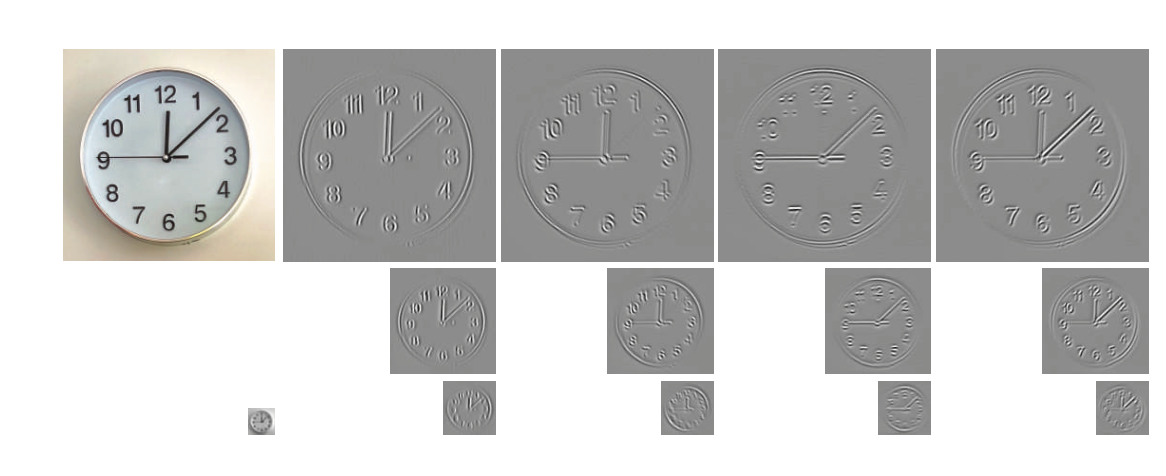
\includegraphics[width=1\linewidth]{figures/pyramids/steerable_pyr_clock.eps}
}
\caption{Steerable pyramid representation (3 levels and 4 orientations). Why is that each orientation subband seems to indicate a different time?}
\label{fig:steerpyr}
\end{figure}


%\begin{figure}[h!]
%\centerline{
%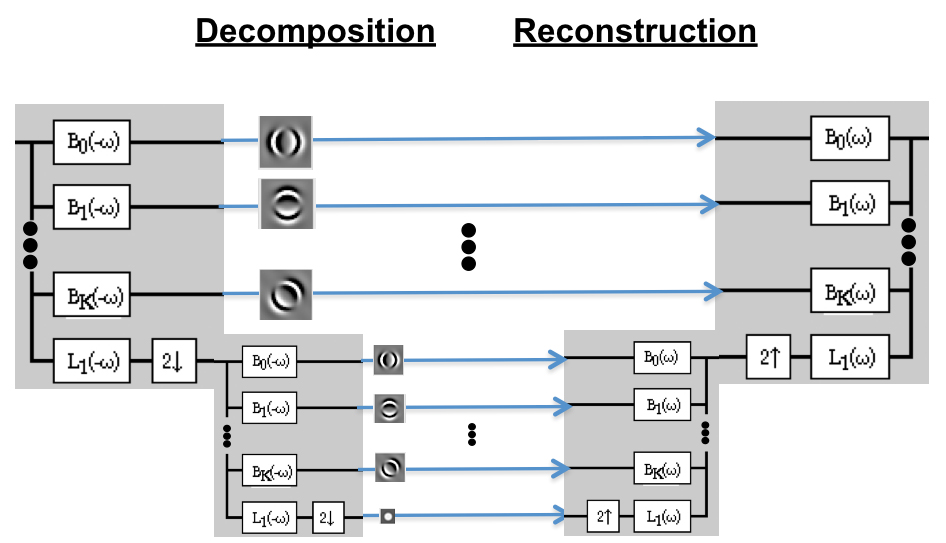
\includegraphics[width=0.7\linewidth]{figures/pyramids/blocksteerpyr.jpg}
%}
%\caption{Steerable pyramid block diagram.}
%\label{fig:blocksteerpyr}
%\end{figure}
%
%


% From Eero toolbox:
%%The steerable pyramid is a multi-scale representation that is
%% translation-invariant, but that also includes representation of
%% orientation.  Furthermore, the representation of orientation is
%% designed to be rotation-invariant. The basis/projection functions
%% are oriented (steerable) filters, localized in space and frequency.
%% It is overcomplete to avoid aliasing.  And it is "self-inverting"
%% (like the QMF/Wavelet transform): the projection functions and 
%% basis functions are identical.  The mathematical phrase for a 
%% transform obeying this property is "tight frame".


%
%
%
%\begin{figure}
%\centerline{
%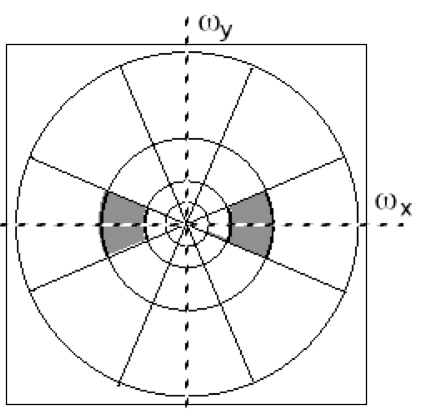
\includegraphics[width=0.4\linewidth]{figures/pyramids/steerpyrfreq.jpg}
%}
%\caption{Steerable pyramid frequency diagram}
%\label{fig:steerpyrfreq}
%\end{figure}
%
%
%There's a mis-match between rotation invariance and the rectangular
%pixel sampling lattice.  The frequency domain is square, but
%a rotationally invariant image representation will have frequency
%subbands arranged as concentric circles, shown in Fig.~\ref{fig:steerpyrfreq}.
%As with the other pyramid image representations, we have a residual,
%unoriented low-pass band, but the steerable pyramid also has a
%high-pass residual subband, as well.
%
%
%\begin{figure}
%\centerline{
%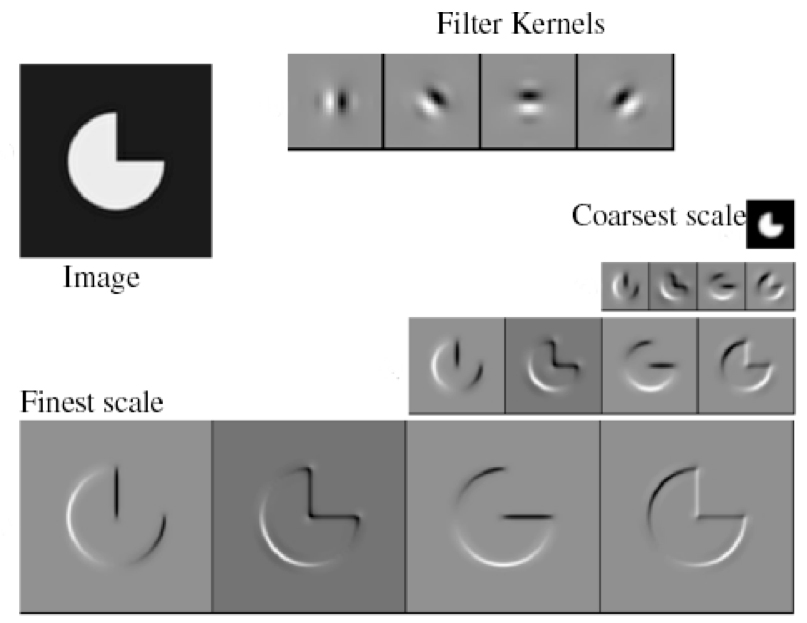
\includegraphics[width=0.7\linewidth]{figures/pyramids/steerpyr.jpg}
%}
%\caption{Steerable pyramid representation.}
%\label{fig:steerpyr}
%\end{figure}
%
%Overall, the steerable pyramid representation is quite overcomplete.
%You can see that in the visualization in Fig.~\ref{fig:steerpyr} of an image and its transform.
%If there are N steerable filters in the representation, then we have N
%images the size of the original at the highest frequency
%representation (plus 1 for the high-pass residual image), and extra
%coefficients are needed to represent the steerable subbands at the
%coarser levels of the pyramid, plus the final low-pass residual image.
%
%So we may not want to use such a representation for image compression
%applications (although the over-complete Laplacian pyramid has been
%used for compression).  But it is useful for various image and texture
%analysis applications, since the subbands represent what they are
%advertised to represent--the signal components in a particular
%frequency band. 
%
%

\section{Concluding remarks}


Here is a pictorial summary of the different pyramid representations we've been discussing in this chapter.  The figure shows the projection matrices $P$ for each transformation in the 1D case.


To recap briefly:  The Fourier transform reveals spatial frequency content of the image wonderfully, but suffers from having no spatial localization. A Gaussian pyramid provides a multi-scale representation of the image, useful for applying a fixed-scale algorithm to an image over a range of spatial scales.  But it doesn't break the image into finer components than simply a range of low-pass filtered versions.  The representation is over-complete that is, there are more pixels in the Gaussian pyramid representation of an image than there are in the image itself.

The Laplacian pyramid reveals what is captured at one spatial scale of a Gaussian pyramid, and not seen at the lower-resolution level above it.  Like the Gaussian pyramid, it is overcomplete. It is useful for various image manipulation tasks, allowing you to treat different spatial frequency bands separately.
%
%A wavelet/QMF pyramid brings in some limited orientation analysis,
%and, different than the other pyramid representations, is complete,
%rather than overcomplete.  This helps it for image compression
%applications, but hurts it for others, since each subband depends on
%information in other subbands to let it reconstruct the original image
%without artifacts.  So if you alter one band without altering the
%corresponding other ones, you can easily introduce artifacts.
%
A steerable pyramid representation can be very overcomplete, depending on the number of orientations represented, but has negligible aliasing artifacts and so can be useful for various image analysis applications.
%
%
%


\begin{figure}
\centerline{
\sublabelnp{1-d Fourier transform}{\includegraphics[width=0.2\linewidth]{figures/pyramids/ftmat.jpg}}
\sublabelnp{1-d Gaussian pyramid}{\includegraphics[width=0.125\linewidth]{figures/pyramids/gmat.jpg}}
\sublabelnp{1-d Laplacian pyramid}{\includegraphics[width=0.125\linewidth]{figures/pyramids/lappmat.jpg}}
%\sublabelnp{1-d Haar pyramid}{\includegraphics[width=0.1\linewidth]{figures/pyramids/haarmat.jpg}}
\sublabelnp{Steerable pyramid}{\includegraphics[width=0.19\linewidth]{figures/pyramids/steermat.jpg}}
}
\caption{Visual comparison of linear transform image representations
  discussed in this chapter.  The Fourier transform gives a
  complex-valued output (represented in color) and is global--each
  output coefficient depends, in general, on every input pixel.  The
  Gaussian pyramid is seen to be banded, showing that it is a
  localized transform where the output values only depend on pixels in
a neighborhood.  It is an over-complete representation, shown by the
transform matrix being taller than it is wide.  
The Laplacian pyramid
is a bandpassed image representation, except for the low-pass residual
layer, shown in the bottom rows. For this matrix, zero is plotted as
grey.  The Haar pyramid is an example of a complete (not
over-complete) representation, so its matrix is square.  The steerable
pyramid is an over-complete, multi-orientation representation.  In 1-d, image orientation
isn't defined, but we show schematically a rasterization of the 2-d
steerable pyramid transform.  The multiple orientations, and
non-aliased subbands cause the representation to be very overcomplete,
much taller than it is wide.
All the transforms,
except for the Fourier transform, are convolutional, revealed by the
diagonal banding in the matrices. 
}
\label{fig:steerpyr}
\end{figure}




%\section{Scale space}






